\section[Introduction]{Introduction\protect\footnote{Sections of this chapter appear in a manuscript submitted to Springerlink as part of the International Conference on Computational 
Science (ICCS) 2025 in the Computing and Data Science for Materials Discovery and Design track, submission number 259 and is
reproduced with permission of Palgrave Springer Nature.}}

% [author and/or editor(s) of contribution], [volume and/or contribution title], [year of publication], [publisher (as it appears on our copyright page)] \

Emulsions can adopt a variety of microstructures depending on fluid volume fractions and the affinity of stabilizing agents for each phase. Among these, bicontinuous 
interfacially jammed emulsion gels (bijels) are characterized by a tortuous, co-continuous network of immiscible fluid domains stabilized by colloidal particles. This 
unique architecture lends itself to numerous advanced applications, including membrane fabrication, catalyst supports, battery electrodes, and pharmaceutical delivery 
systems. Bijels form through the arrest of spinodal decomposition in partially miscible fluid mixtures: as phase separation proceeds, the interface sweeps through the 
system, adsorbing particles until the interfacial area becomes saturated, resulting in jamming. Microstructural features such as domain size, continuity, and interfacial 
curvature critically influence material performance, affecting properties like mass transport, mechanical stability, and surface reactivity. Since their discovery via 
simulation and subsequent experimental realization, research on bijels has expanded significantly, exploring diverse synthesis conditions and scalable processing methods.

The functional properties of bijels are inherently linked to their internal structure. For instance, lower tortuosities in the direction of ion transport yield improved charge 
rates and cycling stability in battery electrodes \cite{ebner_tortuosity_2014, samdani_bicontinuous_2017}. In liquid-liquid extraction, the characteristic pore length-scale governs 
molecular selectivity \cite{khan_nanostructured_2022}, while in pharmaceutical applications, domain size influences drug release rates and cellular behavior 
\cite{vanoli_bijels_2022, thorson_bijel-templated_2019}. Given the sensitivity of these properties to microstructural characteristics, the ability to dynamically modify bijel 
morphology presents a promising strategy to adapt their behavior in situ for targeted performance. In this context, stimuli-responsive emulsions have garnered increasing interest 
for applications requiring dynamic control over material properties, such as enhanced oil recovery, reaction separation, and therapeutic delivery 
\cite{tham_magnetophoresis_2021, cui_stabilizing_2013, rozynek_opening_2019, lu_controllable_2020}. 

These systems can be operated by using external stimuli to alter interfacial configurations, 
enabling modulation of permeability, interfacial area, and morphology. For example, in emulsions stabilized by spherical particles, electric fields can induce droplet deformation via 
particle unjamming and migration before re-establishing interfacial jamming \cite{cui_stabilizing_2013}. Among various stimuli, magnetic fields are particularly attractive due to their 
remote addressability, material compatibility, and bio-relevance. Core-shell ferrite-hydroxyapatite nanorods, for instance, exhibit reversible morphological changes depending on initial 
particle orientation and field direction \cite{nakayama_stimuli-responsive_2018}. In magnetically stabilized Pickering emulsions, magnetophoresis has been shown to drive particle migration 
and interfacial distortion or collapse \cite{tham_magnetophoresis_2021, yang_rapid_2020, misra_magnetic_2020}. Chapter 4 demonstrated that magnetic fields applied during bijel formation can 
bias domain coarsening, producing anisotropic microstructures via orientation-specific jamming \cite{karthikeyan_formation_2024}. However, the structural response of bijels to magnetic fields 
after formation remains poorly understood, presenting an opportunity to explore how external fields may be used to dynamically reconfigure established bijel architectures.

This study investigates the post-formation structural response of bijels stabilized by ellipsoidal magnetic particles under the influence of externally applied magnetic fields. 
Using a hybrid Lattice Boltzmann Method coupled with Molecular Dynamics, we simulate the formation and evolution of bijel structures stabilized by rod-like particles modeled as 
magnetic dipoles. We find that increasing the applied magnetic field after formation induces microstructural changes characterized by increased domain anisotropy and 
coarsening, up to a saturation threshold. In contrast, decreasing or removing the magnetic field results in minimal morphological change, suggesting that the structure is
resilient to removal of stimuli. Analysis reveals that particle unjamming, reorientation at the interface, and subsequent re-jamming are responsible for these structural transformations.
These findings demonstrate how magnetic field manipulation, in combination with ellipsoidal particle stabilization, enables tunable, on-demand microstructure 
control in bijels, offering new capabilities for adaptive material design.

% To understand the saturation behavior, we applied magnetic fields of varying strength to bijel templates formed under increasing initial field conditions. We observed that 
% a greater initial nematic order parameter negatively correlated with the extent of microstructure change. Finally, switching off the magnetic field in pre-aligned bijels had little 
% impact on the microstructure, indicating that the jammed interfacial network prevents reversal of anisotropic features. 

\section{Results}
% \section[Results]{Introduction\protect\footnote{Sections of this chapter appear in a manuscript submitted to Springerlink as part of the International Conference on Computational 
% Science (ICCS) 2025 in the Computing and Data Science for Materials Discovery and Design track, submission number 259 and is
% reproduced with permission of Palgrave Springer Nature.}}
% \label{sec:results_p2}

\subsection{Kinetic arrest}
\label{section:hysteresis_curve}

Bijels have proposed applications as soft-matter-based material templates, drug delivery vectors, and separation systems. In all cases, material performance is 
tightly coupled to the internal microstructure of the bijel template. Applications that benefit from adaptive permeability or structural tunability would be 
enhanced by the ability to reversibly modulate microstructure in situ. This section explores whether magnetically responsive bijels can undergo reversible 
structural changes upon repeated application and removal of an external magnetic field.

We begin by analyzing bijels stabilized by prolate ellipsoidal particles at a particle volume fraction of \(\phi_p = 0.1\). This system is selected due to the 
similar qualitative response mechanisms observed for both prolate and oblate geometries in preliminary simulations (Aim 1), with prolate particles chosen here 
for their greater experimental accessibility. The bijel is initially formed without a magnetic field. After equilibration, a static magnetic field is applied 
in the \(z\)-direction and incrementally increased: \(\bar{B}_z = 0 \rightarrow 0.2 \rightarrow 0.5 \rightarrow 1\). This is followed by a symmetric 
decrement: \(\bar{B}_z = 1 \rightarrow 0.5 \rightarrow 0.2 \rightarrow 0\). At each step, the system is allowed to evolve to a new equilibrium, defined as
the plateauing of the length scale obtained from the domain size, \(L\), computed from the first moment of the spherically averaged structure factor.
\cite{kendon_3d_1999,kendon_inertial_2001} The procedure for the domain size can be found in Equation \ref{eq:spherically_averaged_structure_factor}.

The hysteresis behavior is shown in Figure~\ref{fig:hysteresis_curve}, which plots the normalized domain size \(L/R\) as a function of the applied magnetic 
field at the end of the equilibration step.

\begin{figure} 
    \centering 
    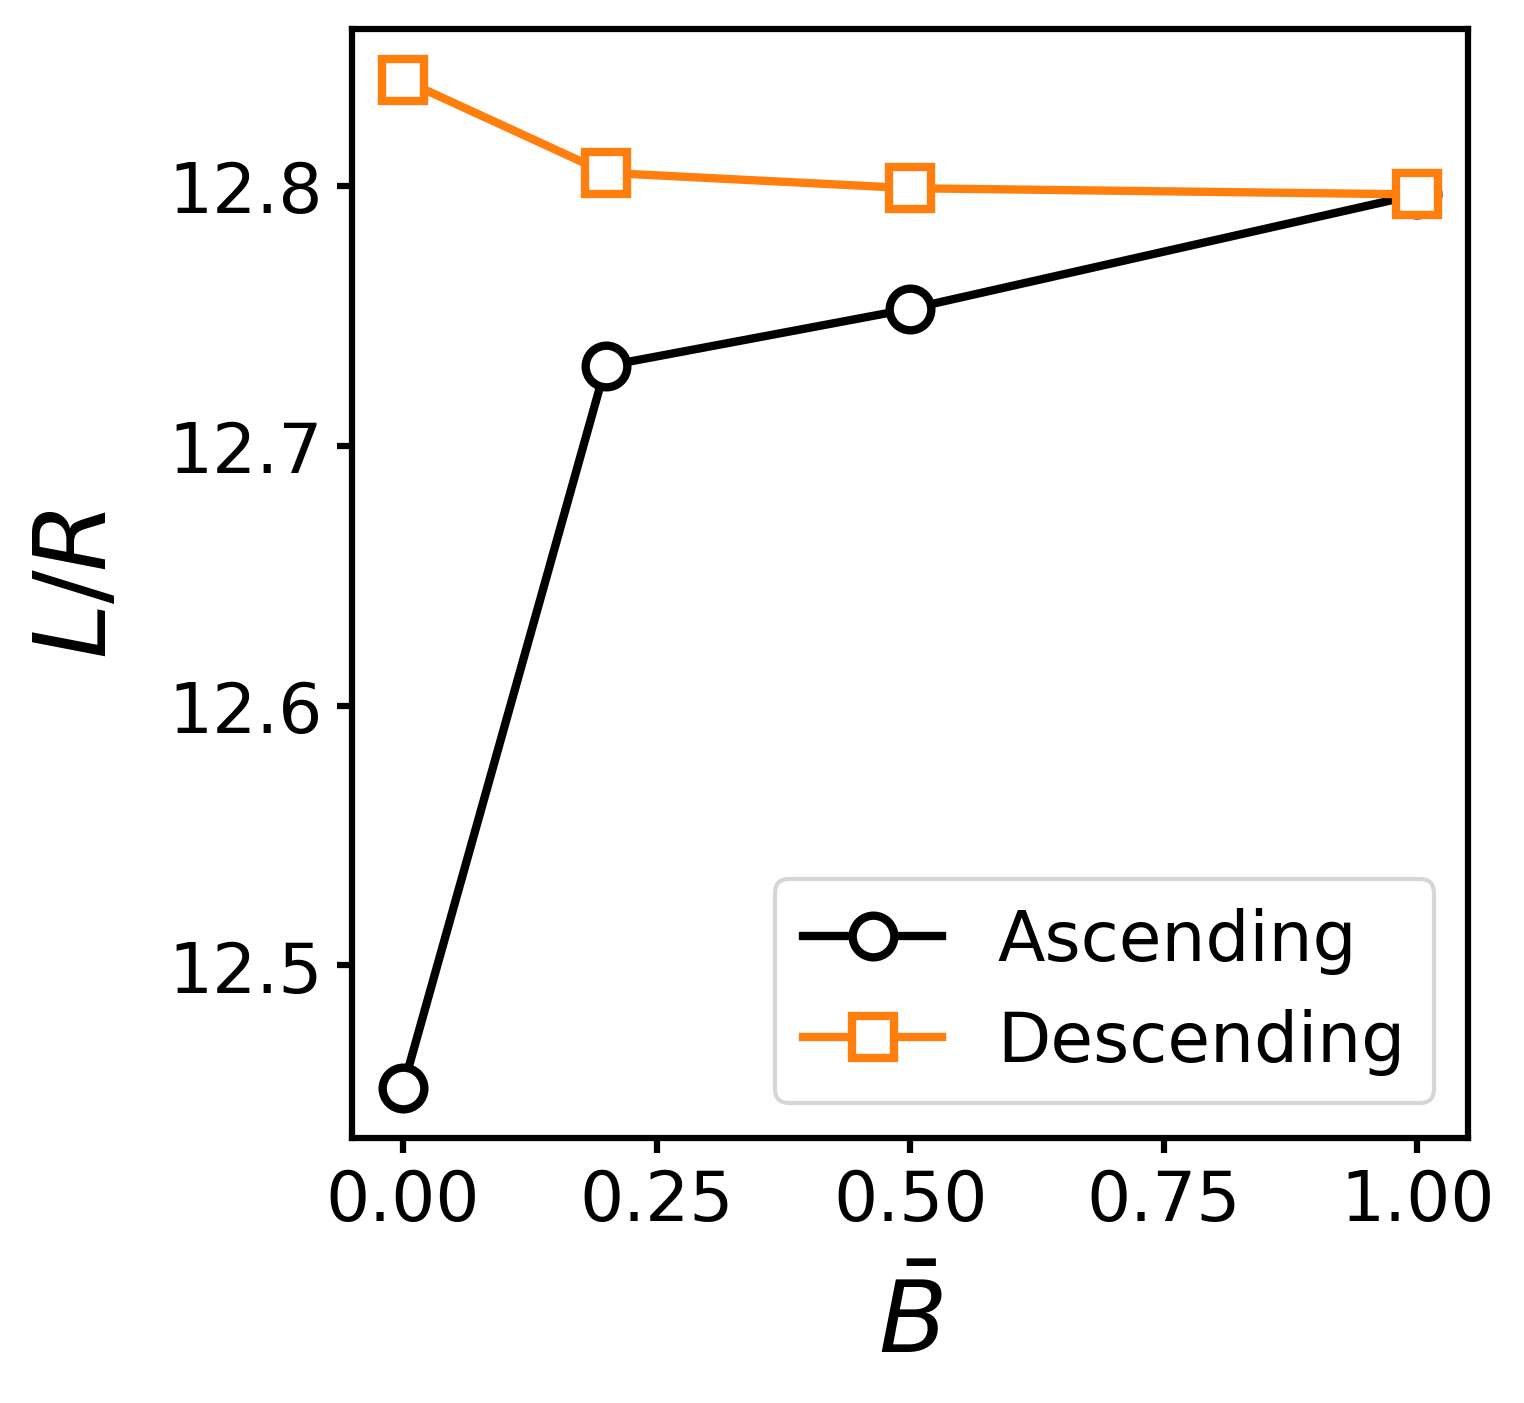
\includegraphics[scale=0.5]{../figures/results/paper2/hysteresis_curve.png} 
    \caption{Plot of the domain size of a bijel stabilized by magnetically responsive prolate particles. We observe that the domain size increases as we 
    increase the applied magnetic field strength. However, upon decrease of the applied field strength the microstructure does not return to its previous value,
    demonstrating kinetic arrest.} 
    \label{fig:hysteresis_curve} 
\end{figure}

The domain sizes characterized in Figure~\ref{fig:hysteresis_curve} demonstrates that as the field is increased, domain size increases, indicating coarsening 
of the fluid domains in the bijel. Chapter 4 showed that application of magnetic fields cause reordering of particles at interfaces towards the
direction of the applied field, enforcing nematic order in the particle monolayer. In the case of already formed bijels,
this reorientation reduces the interface area stabilized, facilitating local unjamming and domain growth. In contrast, when the field strength is reduced, 
the domain size does not revert to its original value, suggesting that the microstructure remains kinetically arrested in the coarsened configuration.

A similar phenomenon has been reported by Cui et al.~\cite{cui_stabilizing_2013} in studies of particle-stabilized emulsions subjected to electric fields, 
where spherical particles unjammed and subsequently rejammed in a new configuration, resulting in anisotropic droplet deformation. Our results extend this 
concept to jammed, bicontinuous systems stabilized by anisotropic particles. Notably, Figure~\ref{fig:hysteresis_curve} also shows that the degree of 
structural change is field-strength dependent, indicating that stronger fields drive more extensive particle reconfiguration. In the following sections, 
we investigate how the magnitude of the applied field and the initial degree of particle ordering influence the extent and reversibility of microstructural 
evolution in magnetically responsive bijels.

\subsection{Applying a field onto a bijel with disordered particles}
\subsubsection{Field strength dependence on domain size}
\label{section:field-strength-dependence-on-domain-size}

The results presented in Figure~\ref{fig:hysteresis_curve} demonstrate that changes in bijel domain size are dependent on the strength of the applied magnetic 
field. in many proposed stimuli-responsive applications, understanding not only the extent but also the mechanism
of structural response is critical for functionality and control. In this section, we investigate the dynamic structural response of bijels stabilized by randomly 
oriented ellipsoidal particles with a volume fraction of \(\phi_p = 0.1\), initially formed without a magnetic field. Magnetic fields of varying strengths 
(\(\bar{B} = 0, 0.2, 0.5, 1\)) are applied to these pre-formed structures to assess how the microstructure evolves under external stimuli. We begin by visualizing 
the microstructure of bijels stabilized by prolate particles before and after field application.

\begin{figure} 
\centering 
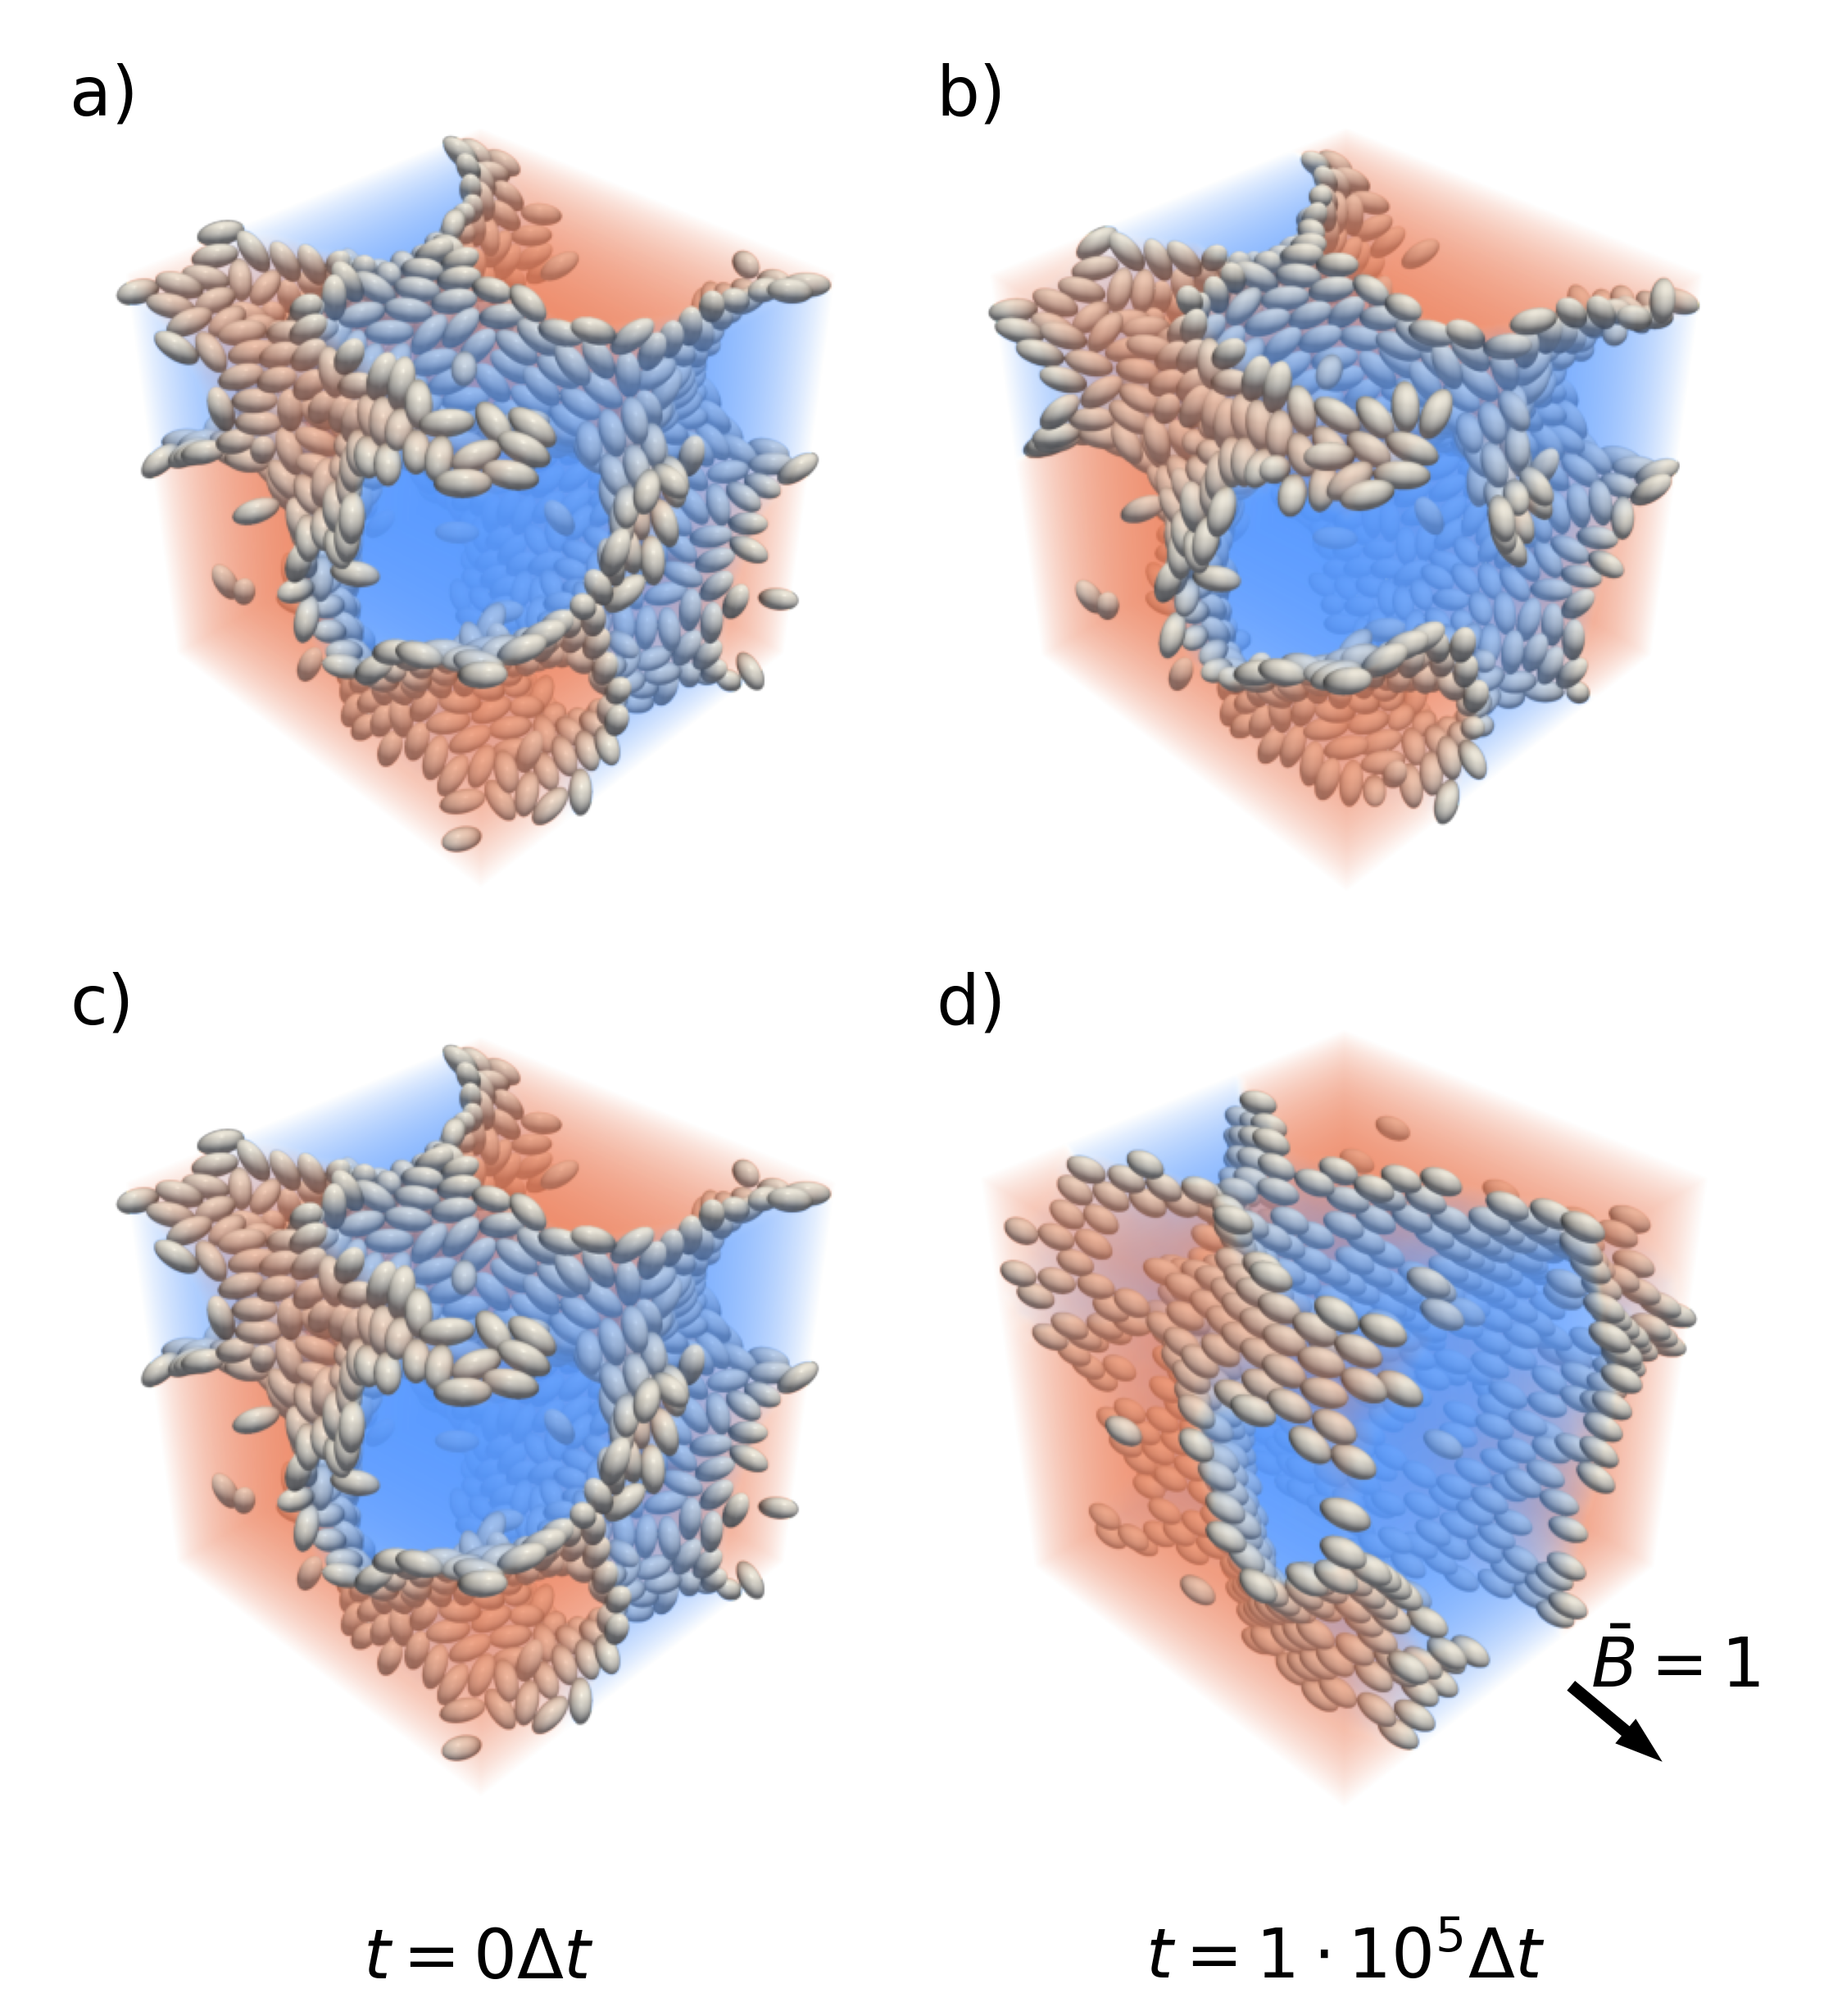
\includegraphics[scale=0.5]{../figures/results/paper2/microstructure_viz-field_on.png} 
\caption{Visualizations of bijels stabilized by prolate particles simulated under no fields at $t = 0$ (left columns) and $t = 10^5$ (right columns). The top 
         row detail the microstructure evolution for bijels with no applied field while the bottom rows show bijels stabilized by oblate and prolate particles 
         respectively with a field strength of $\bar{B} = 1$ applied.}
\label{fig:microstructure_viz-field_on} 
\end{figure}

Figure~\ref{fig:microstructure_viz-field_on} shows that at zero field, the fluid domains exhibit an isotropic, co-continuous morphology with particles randomly 
distributed and oriented at the fluid interface. Upon applying a magnetic field (\(\bar{B}_z = 1\)), the particles undergo reorientation along the field direction, 
which visibly alters the interfacial configuration and the domain morphology. 
To quantitatively characterize this response, we compute the average domain size as a function of time and magnetic field strength. 

\begin{figure} 
    \centering 
    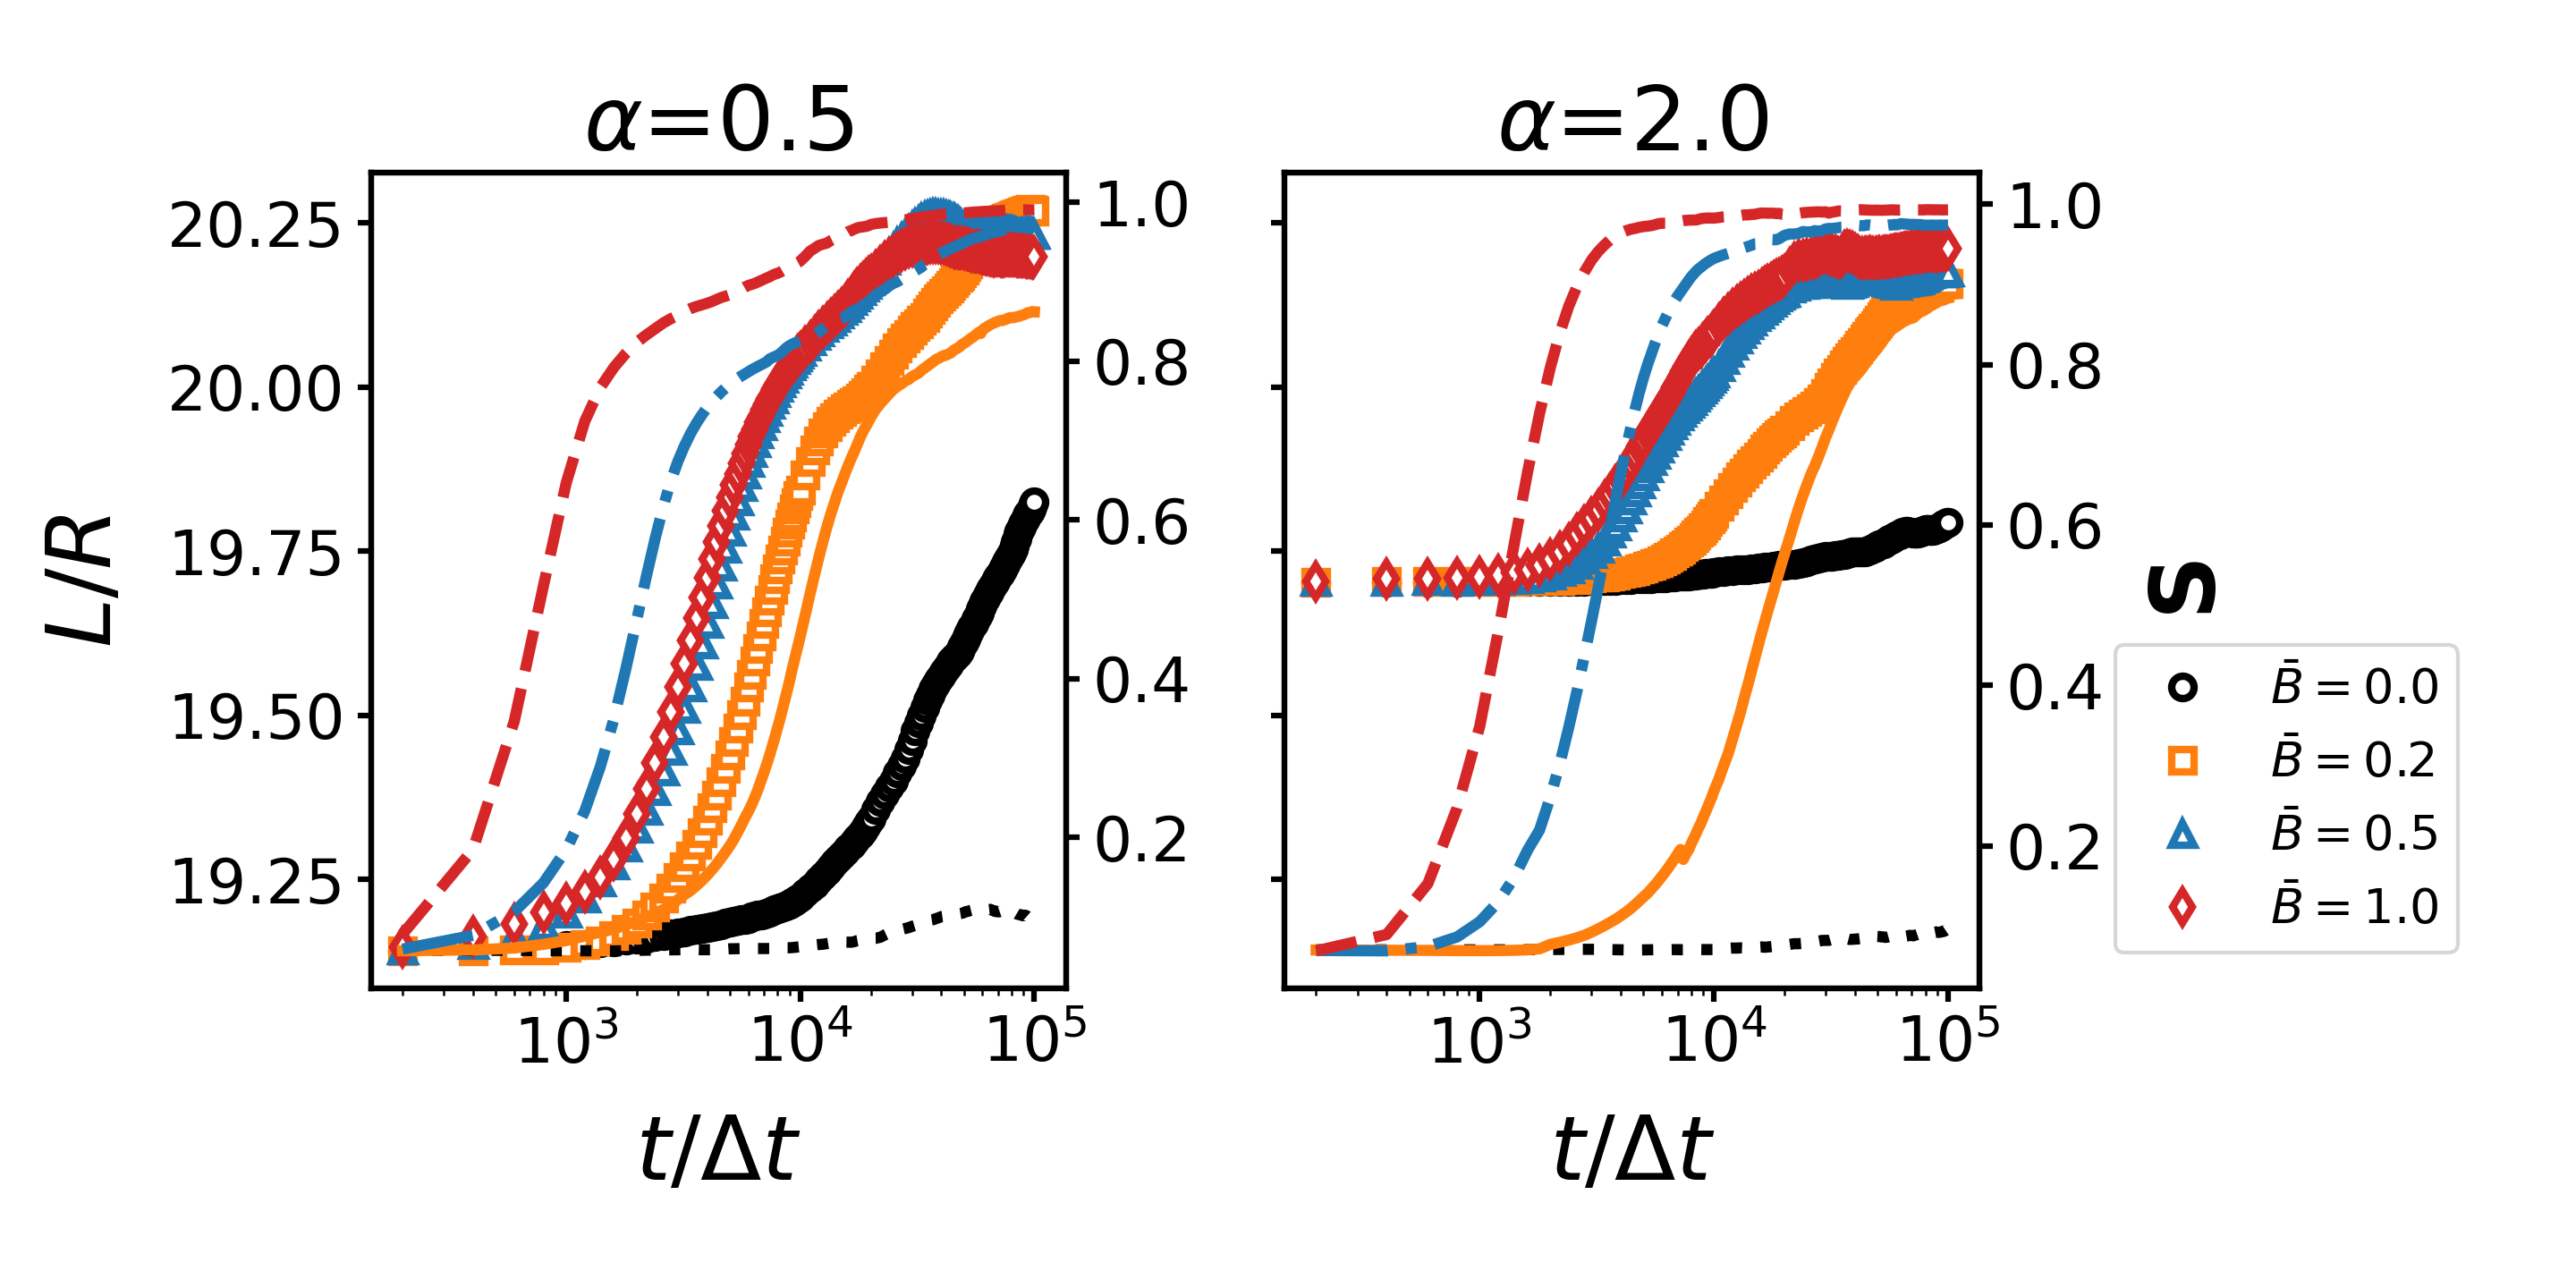
\includegraphics[scale=0.6]{../figures/results/paper2/domain_size-field_on.png} 
    \caption{Plots of the time evolution of the normalized domain size \(L/R\) (markers) for bijels stabilized by oblate (left, \(\alpha = 0.5\)) 
             and prolate (right, \(\alpha = 2.0\)) ellipsoidal particles under varying magnetic field strengths. Here, \(R = 7.9\) is the volume-equivalent sphere radius.} 
    \label{fig:domain_size-field_on} 
\end{figure}

The results show that applying a magnetic field to bijels 
initially formed without one induces domain coarsening, with the final domain size increasing by up to 5.2\% for oblate and 2.5\% for 
prolate particle-stabilized systems.
In both oblate and prolate systems, domain coarsening follows a characteristic three-stage evolution: an initial slow growth phase, a period of rapid 
coarsening, and eventual plateauing as the structure reaches a new jammed configuration. Even in the absence of a magnetic field (\(\bar{B}_z = 0\)), 
domain growth is observed driven by steric rearrangement of interfacial particles, consistent 
with findings by Günther et al.~\cite{gunther_timescales_2014}. 

In Chapter 4, it was identified that the microstructure became anisotropic upon application of magnetic fields. To characterize if the same is observed
when applying a magnetic field onto a formed bijel, we plot the anisotropic domain size and tortuosity as a function of the applied magnetic field. The
directional domain size is calculated using the technique outlined in Equation \ref{eq:directional_structure_factor} and the tortuosity is calculated
using the technique used to generate the data for Figure \ref{fig:tau_B}.

\begin{figure} 
    \centering 
    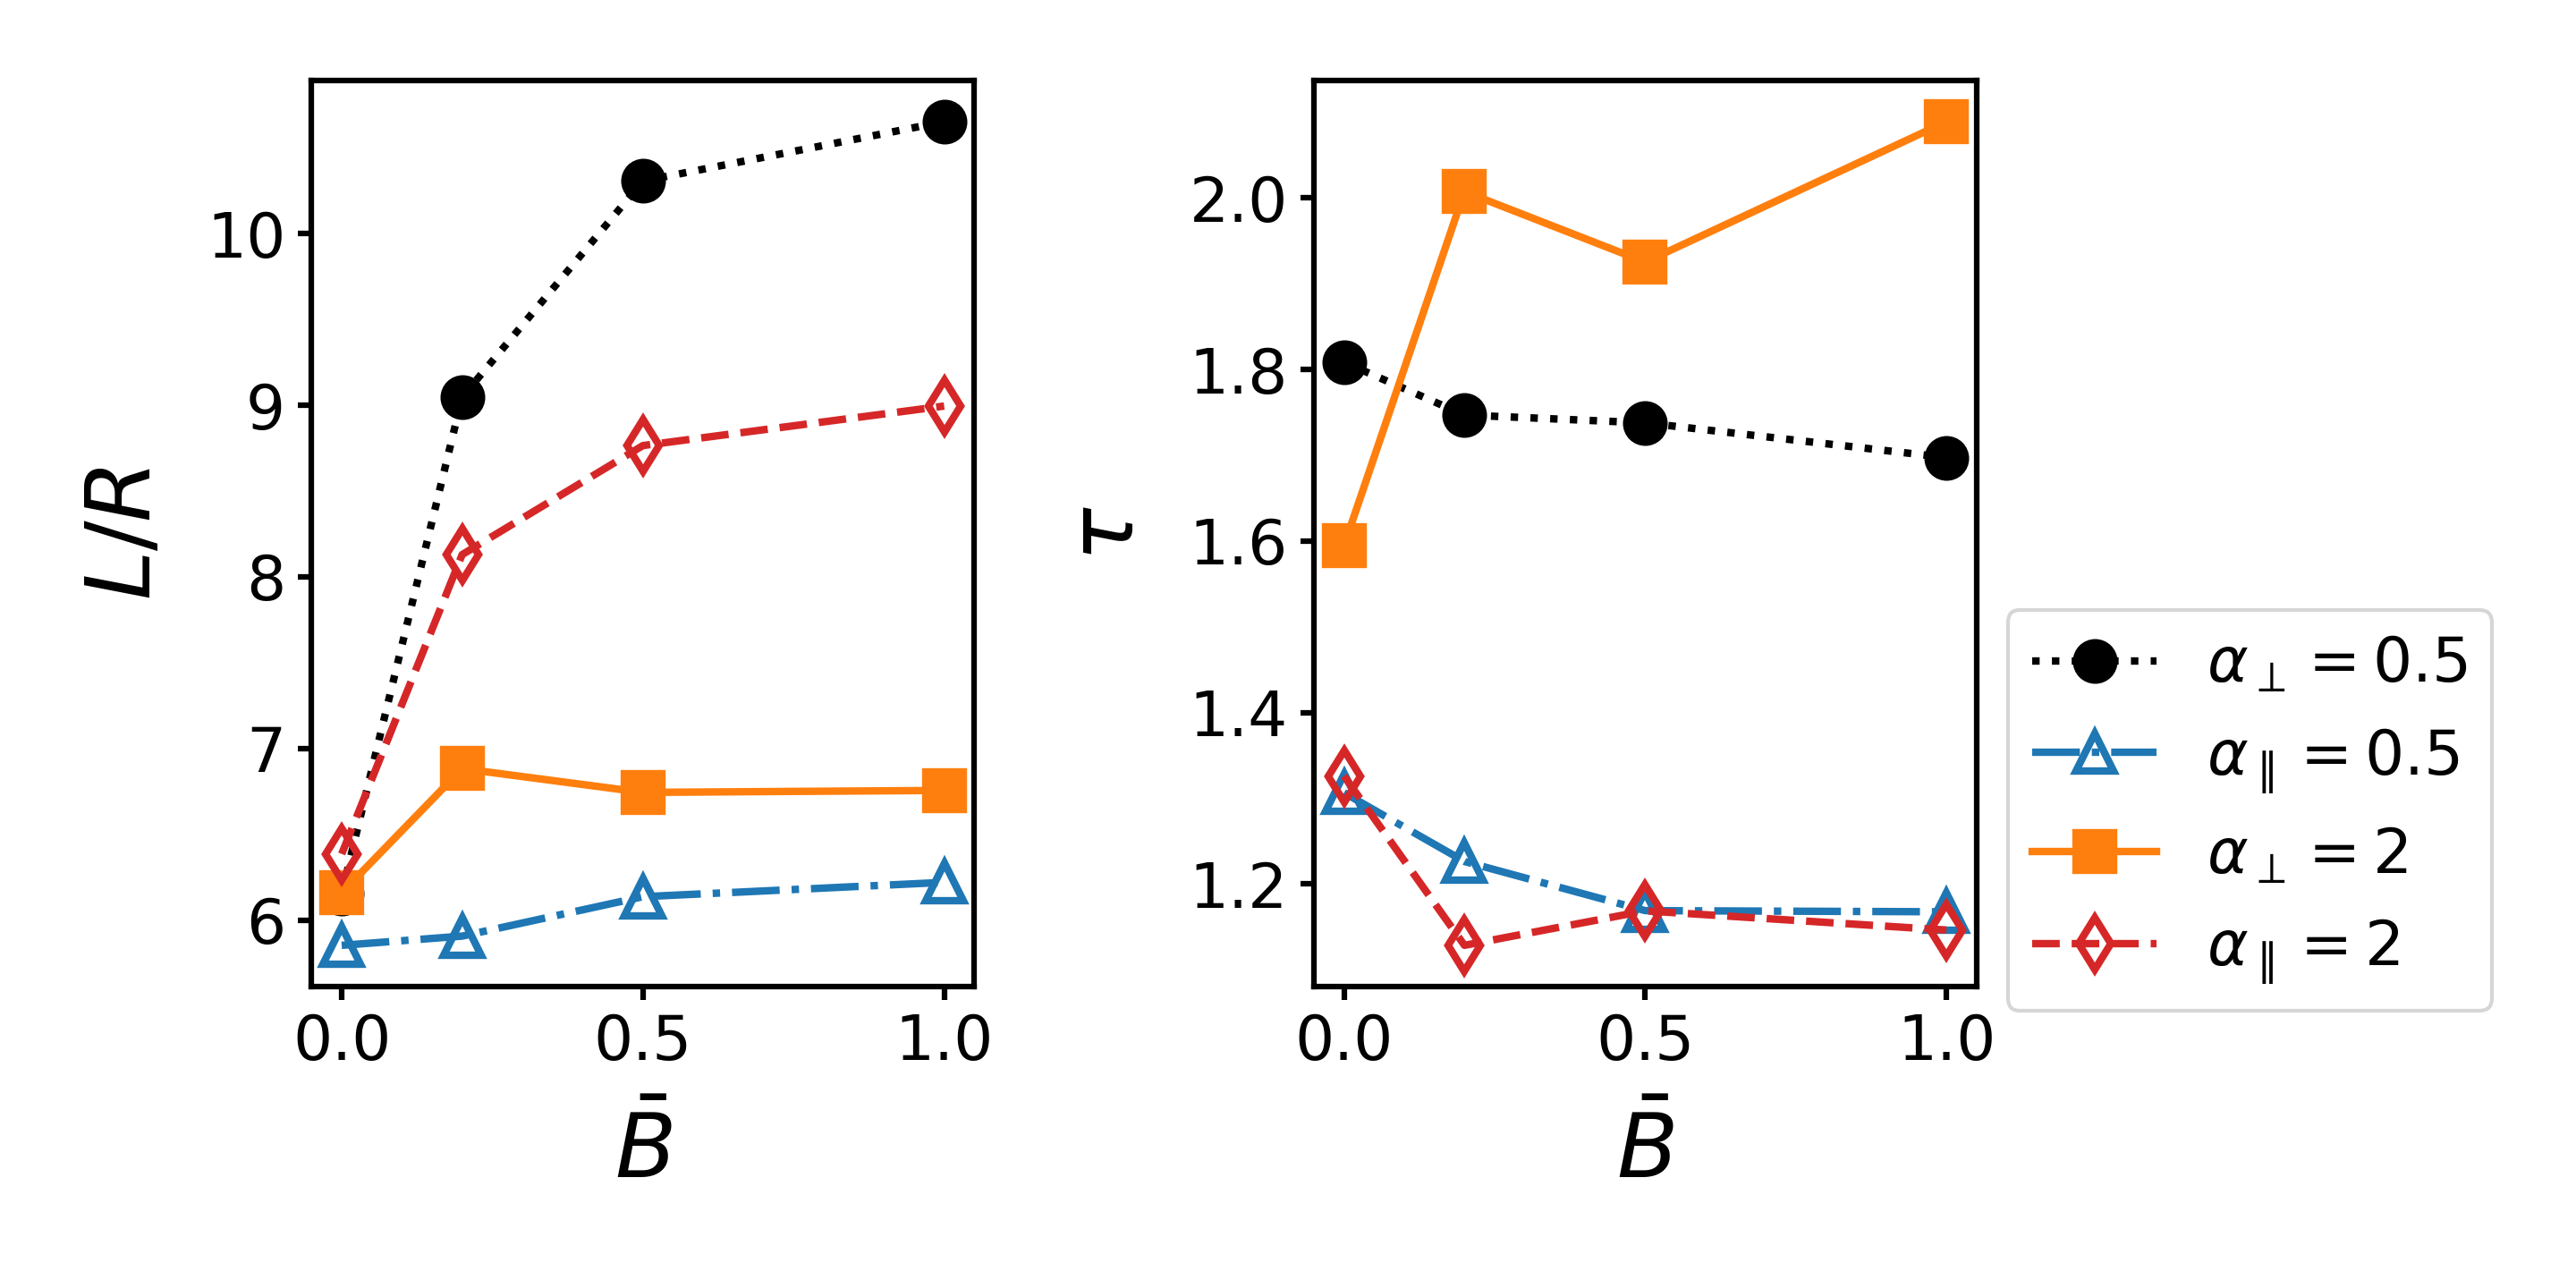
\includegraphics[scale=0.6]{../figures/results/paper2/domain_size_aniso-field_on.png} 
    \caption{Plots of the anisotropic domain size (left) and tortuosity (right) as a function of magnetic field strength for bijels 
             stabilized with oblate and prolate ellipsoids when raising the applied magnetic field. Prolate-stabilized bijels 
             exhibit increased domain size parallel to the field ($L_{\parallel}$) and decreased size perpendicular ($L_{\perp}$), 
             while the opposite trend is observed for oblate-stabilized systems. Tortuosity inversely correlates with domain size in 
             both cases.} 
    \label{fig:domain_size_aniso-field_on} 
\end{figure}

Figure~\ref{fig:domain_size_aniso-field_on} shows that the application of a magnetic field induces domain size anisotropy in bijels stabilized by both oblate 
and prolate particles. Even at zero field, a small degree of anisotropy is observed, which increases substantially with rising field strength. For oblate particles, 
the domain sizes perpendicular (\(L_\perp\)) and parallel (\(L_\parallel\)) to the applied field increase by approximately 73\% and 7\%, respectively. In contrast, 
for prolate particles, \(L_\perp\) increases by 10\%, while \(L_\parallel\) increases by 44\%. These results indicate that the dominant direction of coarsening 
depends on particle morphology: oblate particles promote greater coarsening perpendicular to the field, while prolate particles favor coarsening parallel to the 
field. This trend reflects how particles reorient in response to the applied magnetic field. As particles unjam and rejam 
at the interface, they adopt morphology- and field-dependent orientations that result in directionally biased surface coverage, manifesting as anisotropic domain 
growth.

The right panel of Figure~\ref{fig:domain_size_aniso-field_on} presents the corresponding changes in directional tortuosity. Initially, the tortuosity values 
for both directions are close to \(\tau \approx 1.5\), aligning with previous simulations of gyroidal and co-continuous structures using Lattice Boltzmann methods 
\cite{luo_macroscopic_2020}. Upon applying the magnetic field, \(\tau_\perp\) decreases while \(\tau_\parallel\) increases. This inverse relationship between 
tortuosity and domain size is consistent with prior findings \cite{karthikeyan_formation_2024}, where larger domains exhibited 
reduced tortuosity. The observed anisotropic response suggests that magnetic fields not only influence interfacial particle orientation but also lead to 
direction-dependent transport pathways in the bijel. Moreover, the extent and direction of anisotropy are strongly influenced by the particle morphology, 
particularly the axis of symmetry, which dictates the dominant direction of microstructural reorganization under field application. The time dependence of
the reorientation of particles at the interface is characterized next.

\subsubsection{Particle reorientation at the interface}

The primary effect of the magnetic field is the torque it exerts on the particles' magnetic dipoles, driving them to rotate and align with the field direction. 
This field-induced alignment is clearly evident in the simulation snapshots shown in Figure~\ref{fig:particle_viz-field_on}. In the absence of a magnetic field 
(\(\bar{B} = 0\)), the particles exhibit random orientations at the interface. However, when the field is applied (\(\bar{B} = 1\)), the dipoles display a strong 
degree of orientational order aligned with the field direction.

\begin{figure} 
\centering 
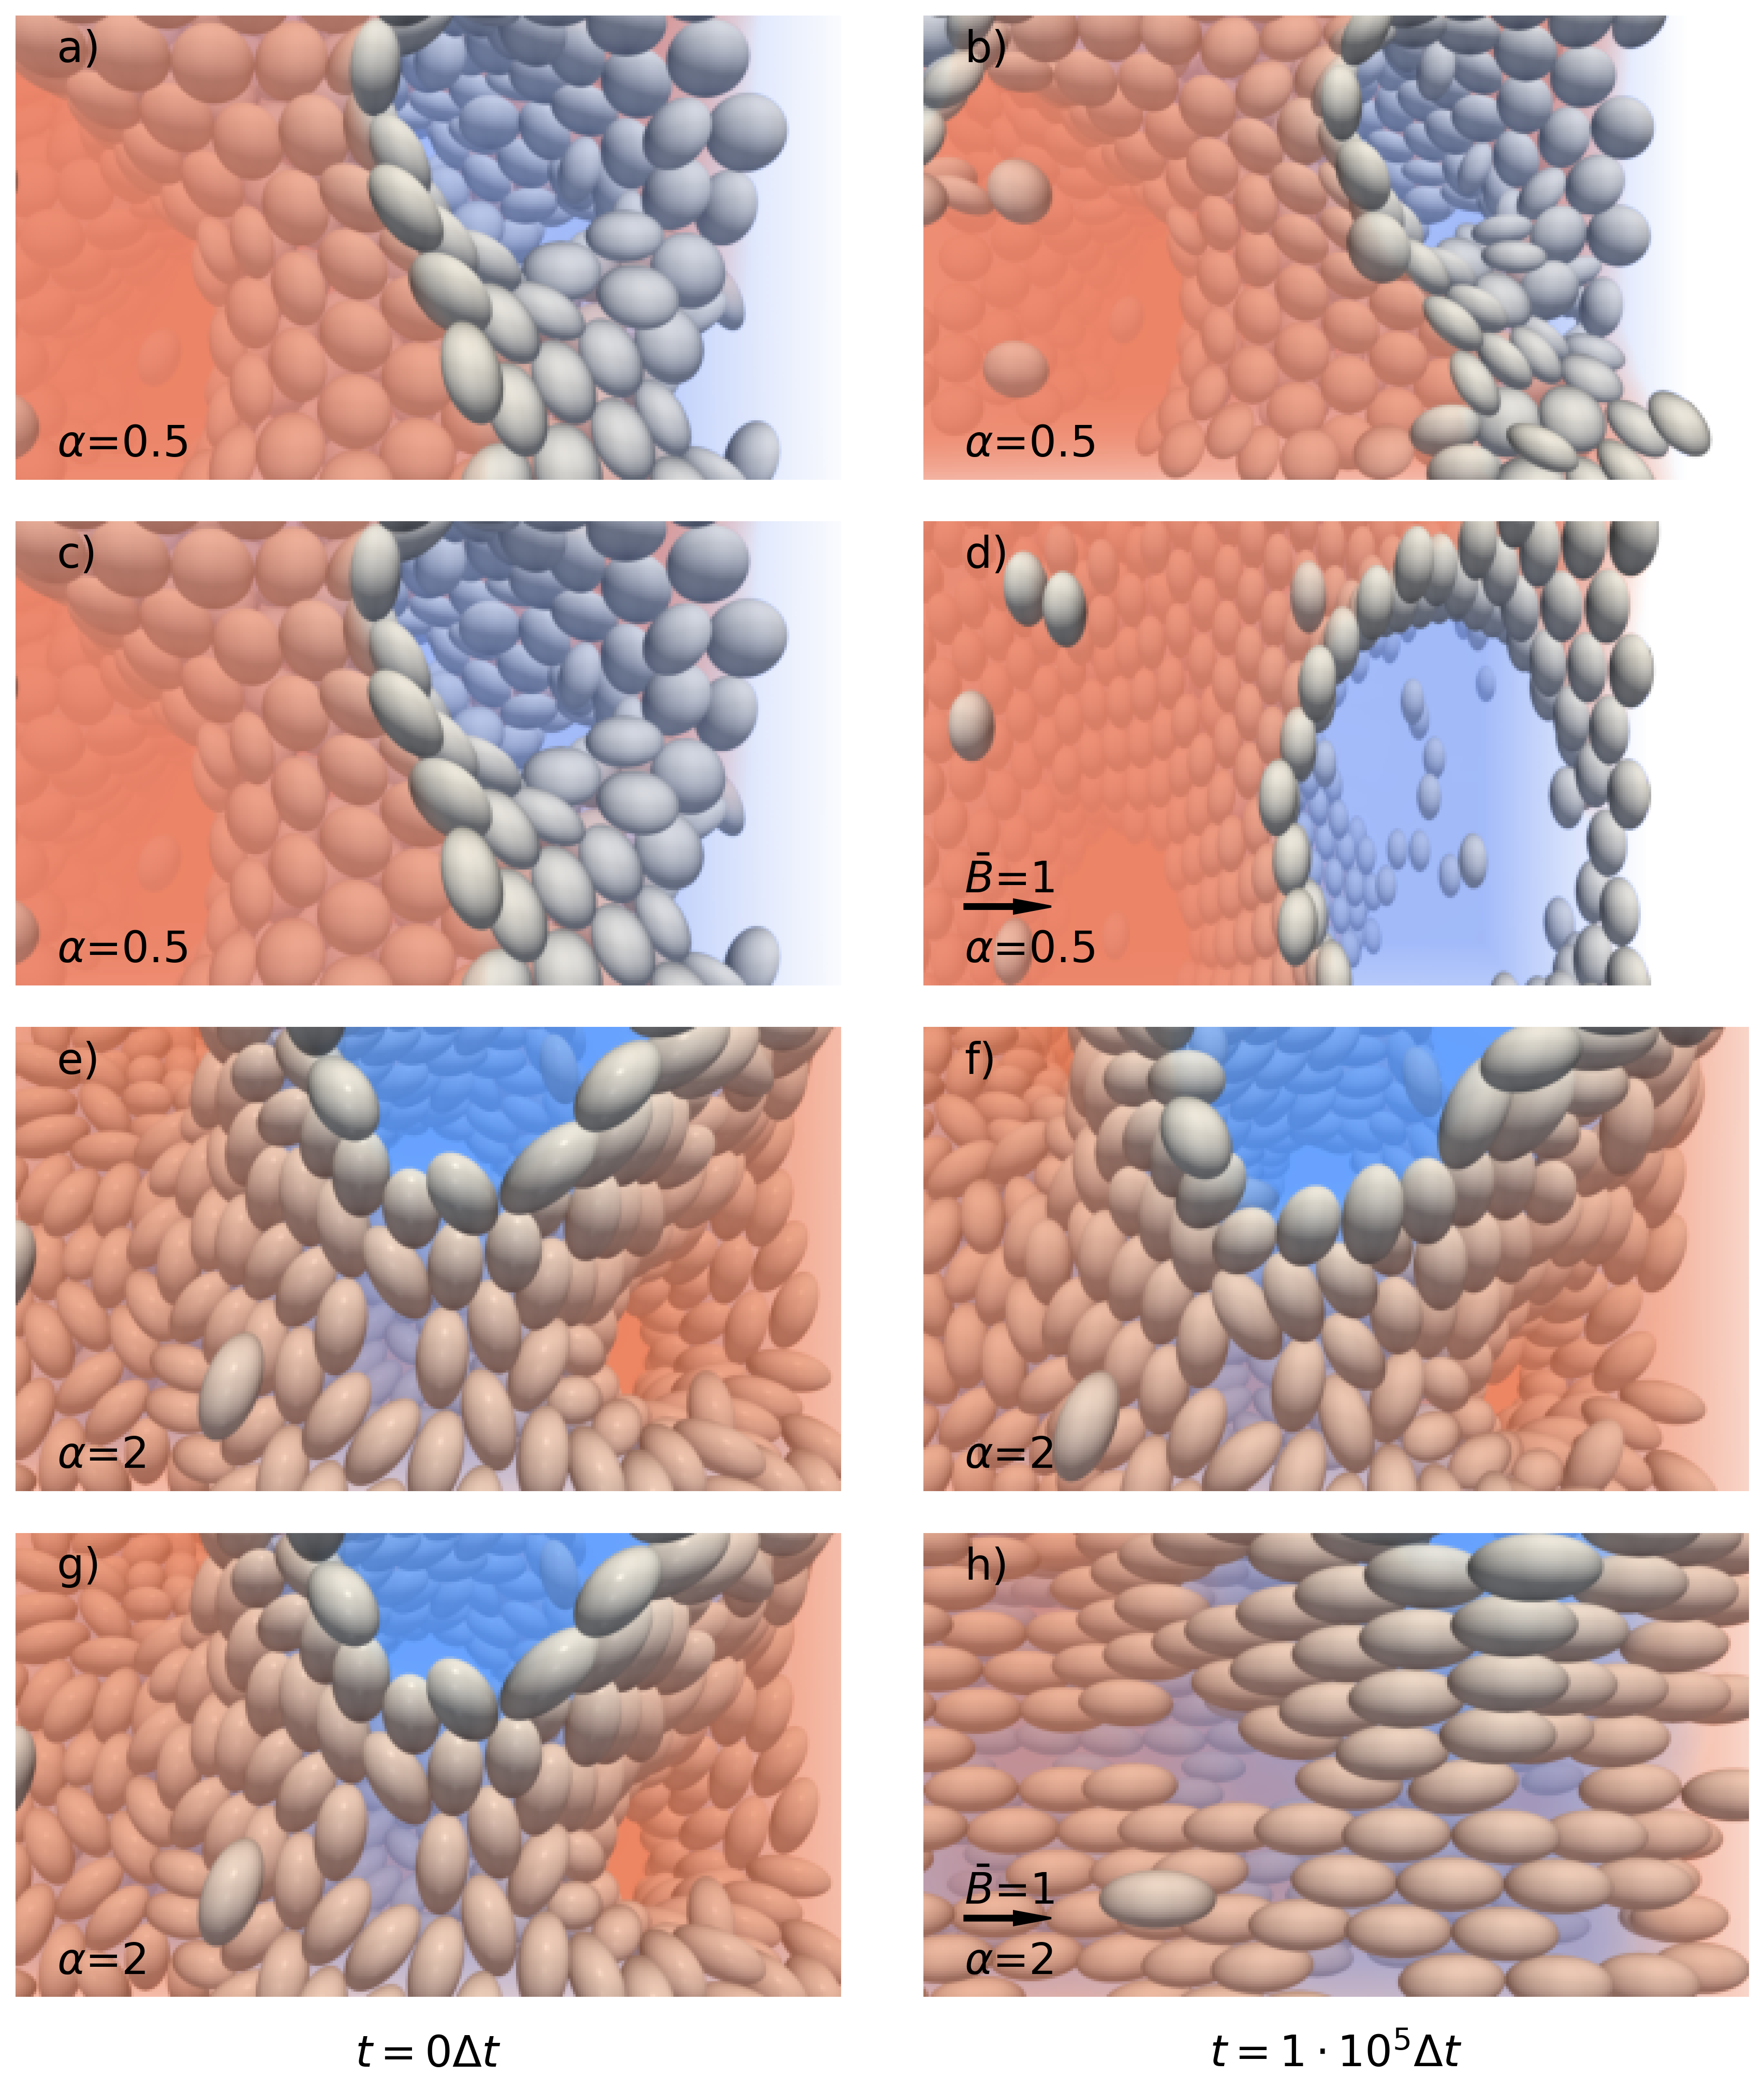
\includegraphics[scale=0.4]{../figures/results/paper2/particle_viz-field_on.png} 
\caption{Visualizations of bijels stabilized by prolate ellipsoidal particles at the initial and final timesteps, 
         both in the absence of a magnetic field (top row) and with a magnetic field applied (\(\bar{B}_z = 1\), bottom row). Particle reorientation to the
         applied field can be observed.} 
\label{fig:particle_viz-field_on} 
\end{figure}

To analyze the reorientation of particles to the magnetic field over time, the nematic order parameter of the particle monolayer is calculated. This is done
in the same technique used for Figure \ref{fig:nematic_time}. 

\begin{figure} 
    \centering 
    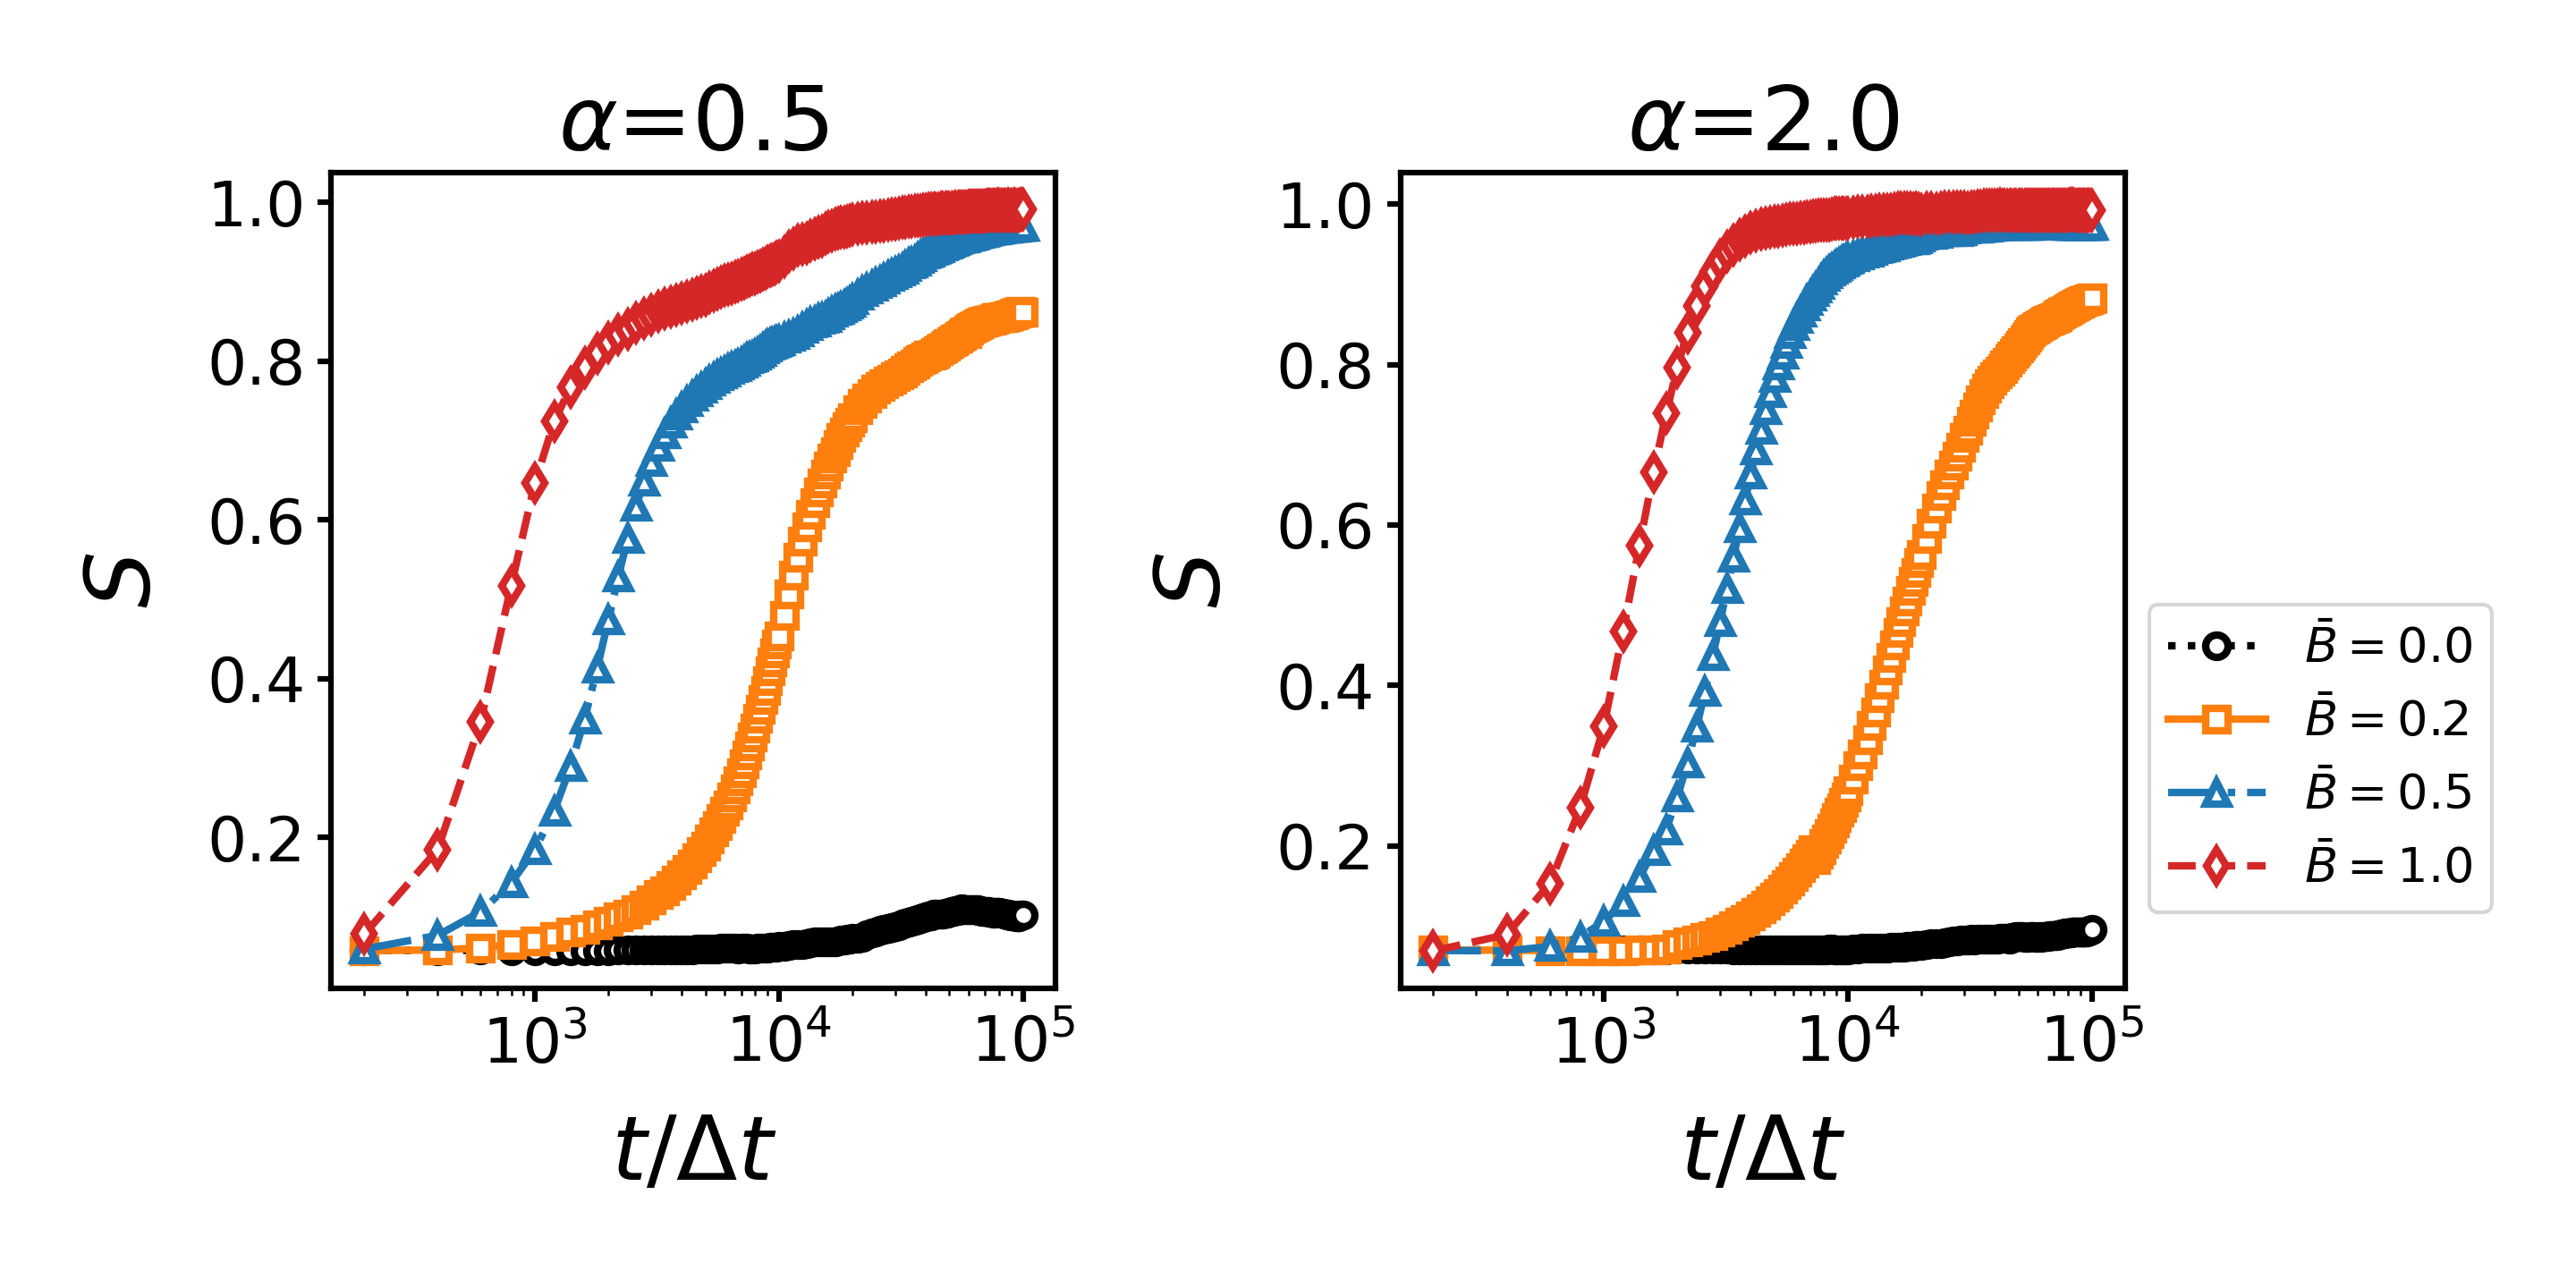
\includegraphics[scale=0.6]{../figures/results/paper2/nematic-field_on.png} 
    \caption{Evolution of the nematic order parameter \( S \) over time for bijels stabilized with disc-like particles (left) and rod-like particles (right), 
             after the application of varying magnetic field strengths.} 
    \label{fig:nematic-field_on} 
\end{figure}

From Figure \ref{fig:nematic-field_on}, as field strength increases, particles exhibit earlier and more pronounced alignment, with \( S \) approaching unity 
for \( \bar{B} = 1.0 \), indicating strong global nematic order. In contrast, systems with no applied field (\( \bar{B} = 0 \)) remain disordered throughout, 
with low \( S \) values. The time-dependent development of nematic ordering reflects the interplay between magnetic torque and interfacial mechanics. 
The increase in \( S \) demonstrates the application of a constant magnetic field causes particle to rotate at the interface to align with the magnetic field.
Linking the alignment of the particles to the domain size change showed in Figure \ref{fig:domain_size-field_on}, the rotation of particles to the magnetic field 
overcomes the initial interfacial jamming. allowing particles to realign to the field. As alignment 
progresses, the particles re-jam. In Chapters 4 and 5, the application of the magnetic field modified the angle of the particle to the interface and the
local packing of the particles. This was caused by orientational of the particles to the magnetic field causing direction dependent cessation of coarsening.
To understand how the rotation of particles affects the particle monolayer, the interfacial angle $\langle \psi \rangle$ is analyzed to understand
how the nematic transition takes place at the interface. $\langle \psi \rangle$ is calculated in the same method as that used to generate Figure \ref{fig:psi_time} 
in Chapter 4, with the results presented in Figure \ref{fig:interface_angle-field_on}. 

% `To understand the interfacial dynamics, the interface angle and the lo This interpretation motivates complementary measurements of the interfacial angle \( \langle \psi \rangle \) and local 
% packing order \( \langle Q_6 \rangle \), which together provide deeper insight into how the transition from disordered to ordered interfacial states is governed by 
% field strength and particle anisotropy.

% The snapshot shows that in the absence of a magnetic field, minor variations in particle orientation and position occur as the bijel is not jammed, as 
% previously observed by Günther et al.~\cite{gunther_timescales_2014}. However, the application of a magnetic field induces clear orientational ordering of the 
% particle monolayer, with particles aligning along the field direction and reorganizing into distinct interfacial arrangements. Newton et al. showed that
% the lowest energy state of arrays of ellipsoidal particles are not at the same orientations to one another when tilted by a magnetic field at an interface.
% \cite{newton_capillary_2018} These changes suggest that both 
% capillary forces and steric hindrance are modified upon field application. While particles naturally prefer to lie flat at the interface to minimize interfacial 
% adsorption energy, the applied field competes with this tendency, reorienting the particles and disrupting their initial packing. The angle of the particle to the
% interface can be used to characterize the reorientation of particles to the magnetic field. The calculation is done in the same way as what is done in Figure
% \ref{fig:psi_time} in Chapter 4.'

\begin{figure} 
    \centering 
    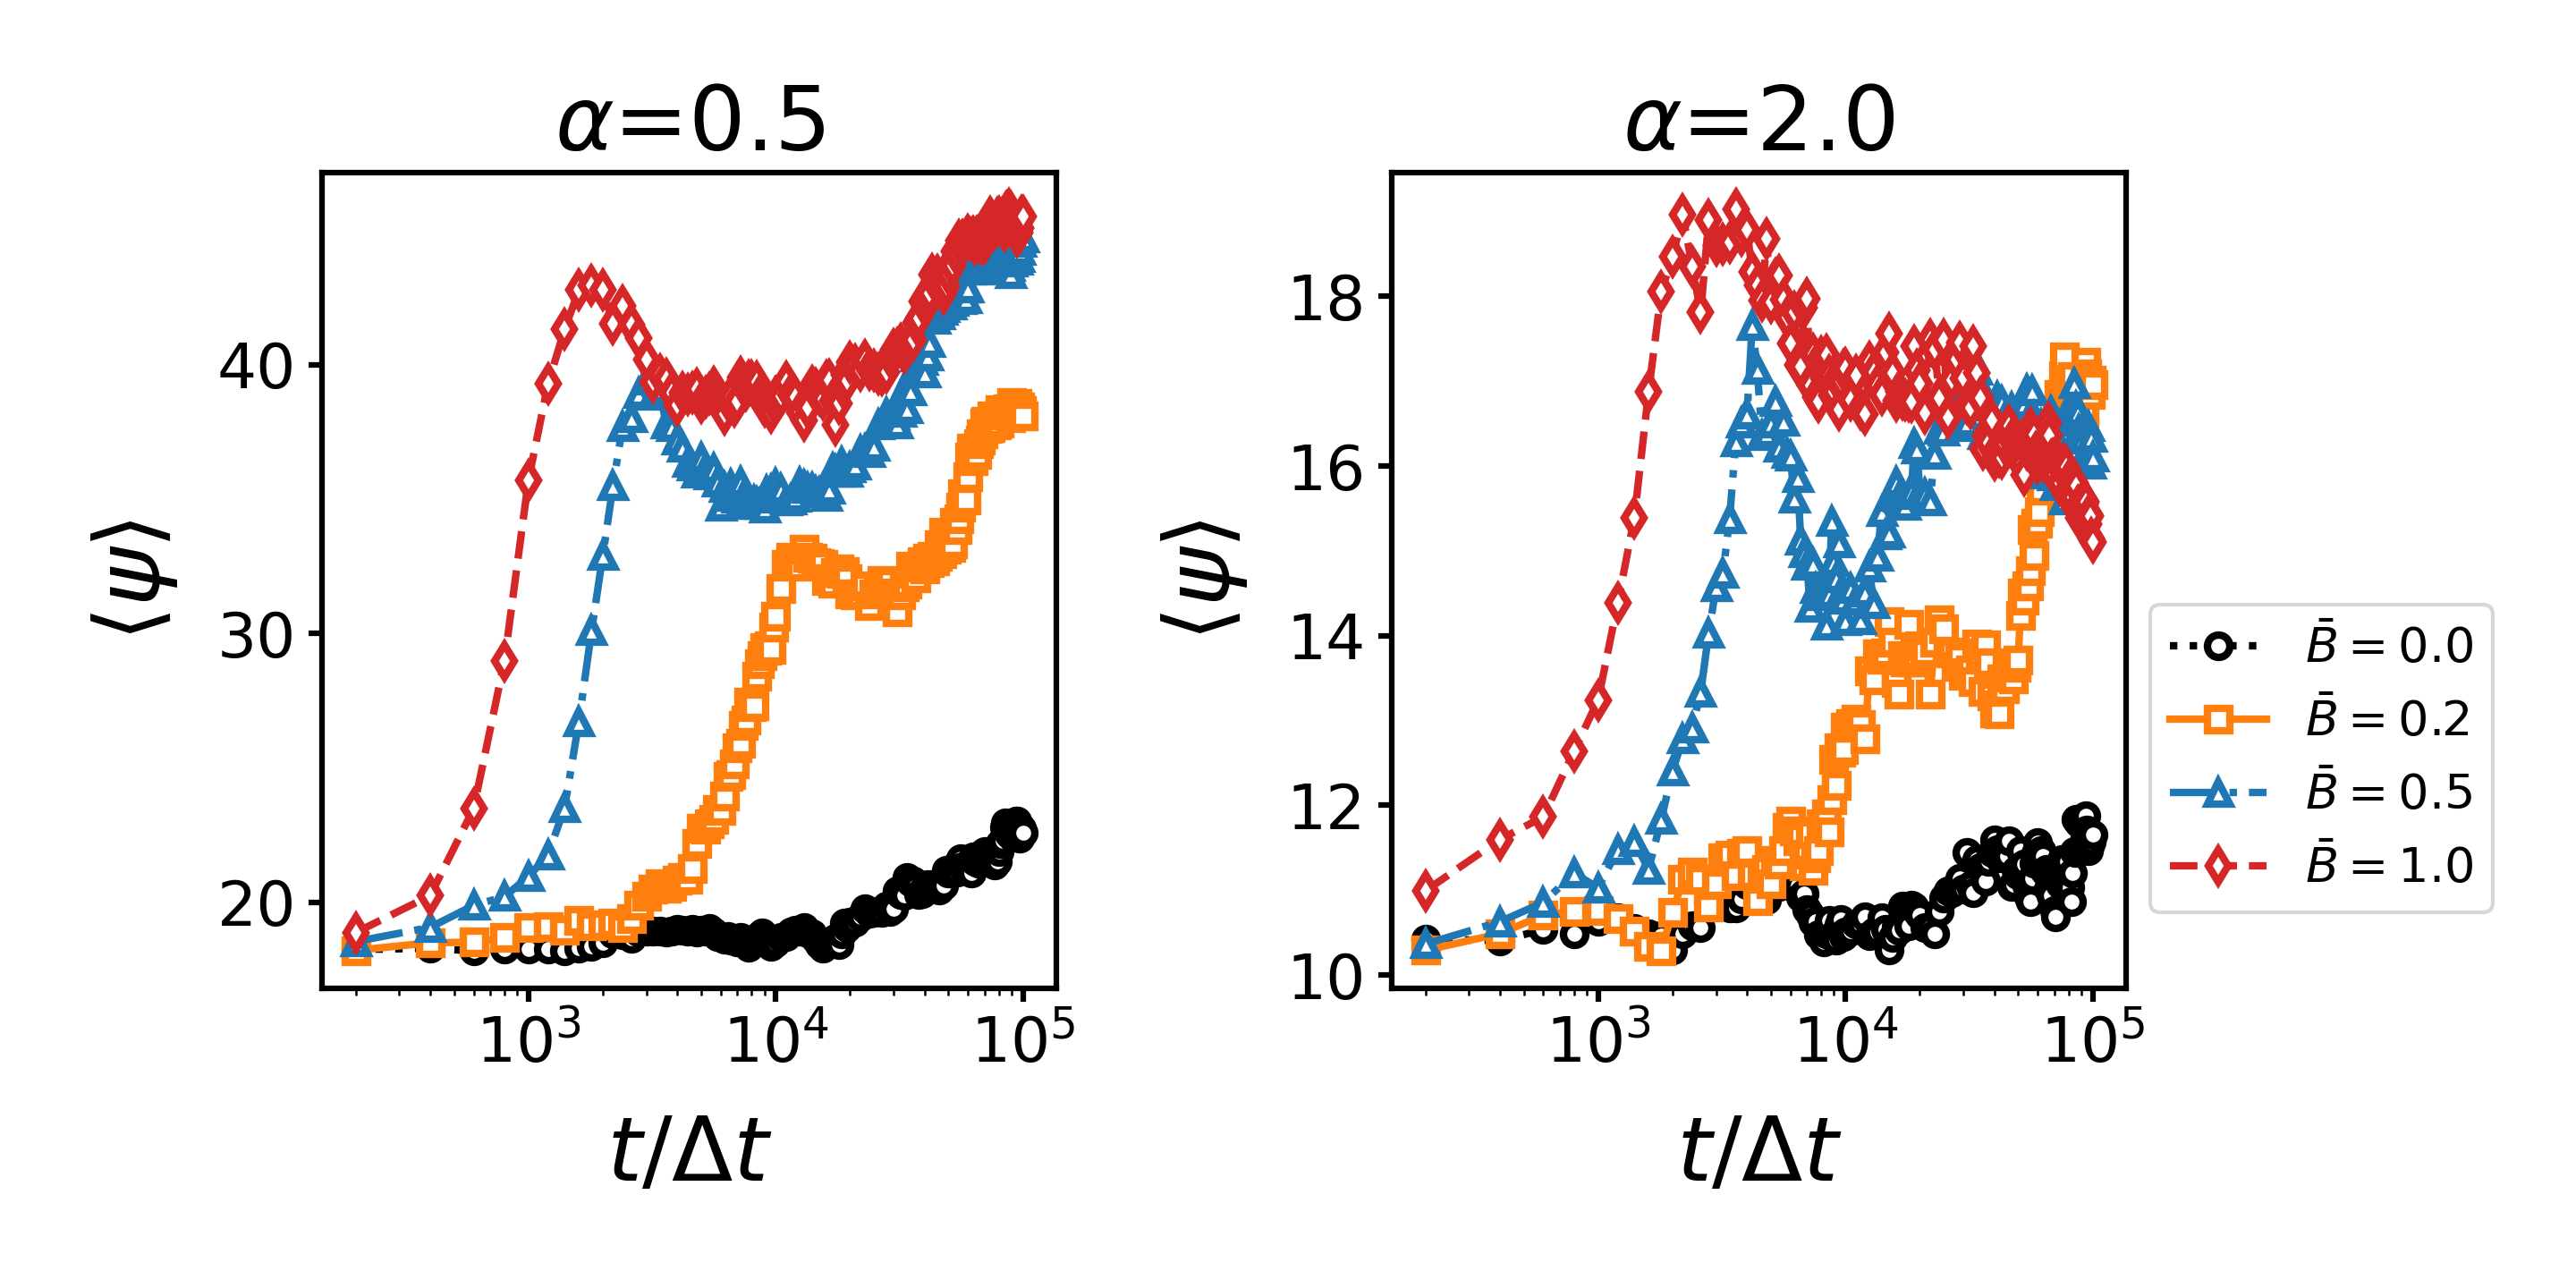
\includegraphics[scale=0.6]{../figures/results/paper2/psi-field_on.png} 
    \caption{Plots of the evolution of the average interface angle \(\langle \psi \rangle\) over time for bijels stabilized 
             by oblate (left) and prolate (right) ellipsoidal particles under varying magnetic field strengths. The response of \(\langle \psi \rangle\) 
             differs notably between the two particle morphologies.} 
    \label{fig:interface_angle-field_on} 
\end{figure}

For bijels stabilized by oblate particles, \(\langle \psi \rangle\) initially increases from approximately \(19^\circ\), indicating that the particles, which begin 
in an approximately flat configuration at the interface, begin to tilt out of the plane in response to the applied field. After a brief decrease or plateau, the angle 
resumes increasing before stabilizing. This behavior suggests that particles first reorient under magnetic torque but are temporarily resisted by interfacial tension 
and capillary constraints. Once the interface begins to deform in response to particle tilt, the system eventually jams in a new configuration, locking the particles 
at an elevated angle. Both the rate of initial tilt and the duration of the plateau phase increase with field strength, and the final value of 
\(\langle \psi \rangle\) is positively correlated with the magnitude of the applied field.

For bijels stabilized by prolate particles, a similar trend is observed. The initial value of \(\langle \psi \rangle\) starts around \(10^\circ\), gradually increases, 
and then exhibits a plateau followed by a slight decline. While the rate and magnitude of the initial increase are field-dependent, the final values converge more 
closely across different field strengths, suggesting that the field sensitivity of interface tilt is weaker for prolate particles. The overall changes in \(\langle \psi \rangle\) 
are also smaller in magnitude compared to those in oblate systems, indicating that prolate particles experience less pronounced reorientation at the interface. This is due to 
the smaller effective lever arm for magnetic torque in prolate particles, which limits their rotational response to the field. 

While the interface angle \(\langle \psi \rangle\) provides insight into the out-of-plane orientation of particles in response to magnetic field application, 
it does not capture how particles reorganize at the interface, observed in Figure \ref{fig:microstructure_viz-field_on} Since the evolution of microstructure is 
influenced not only by tilt but also by the steric effects of interfacial particles, we also assess the Steinhardt bond orientational parameter. The Steinhardt
bond orientational parameter is calculated using the Freud package using the same technique described in Equation \ref{eq:steinhardt_definition}. The results
are plotted in Figure \ref{fig:Q6-field_on}.

\begin{figure} 
    \centering 
    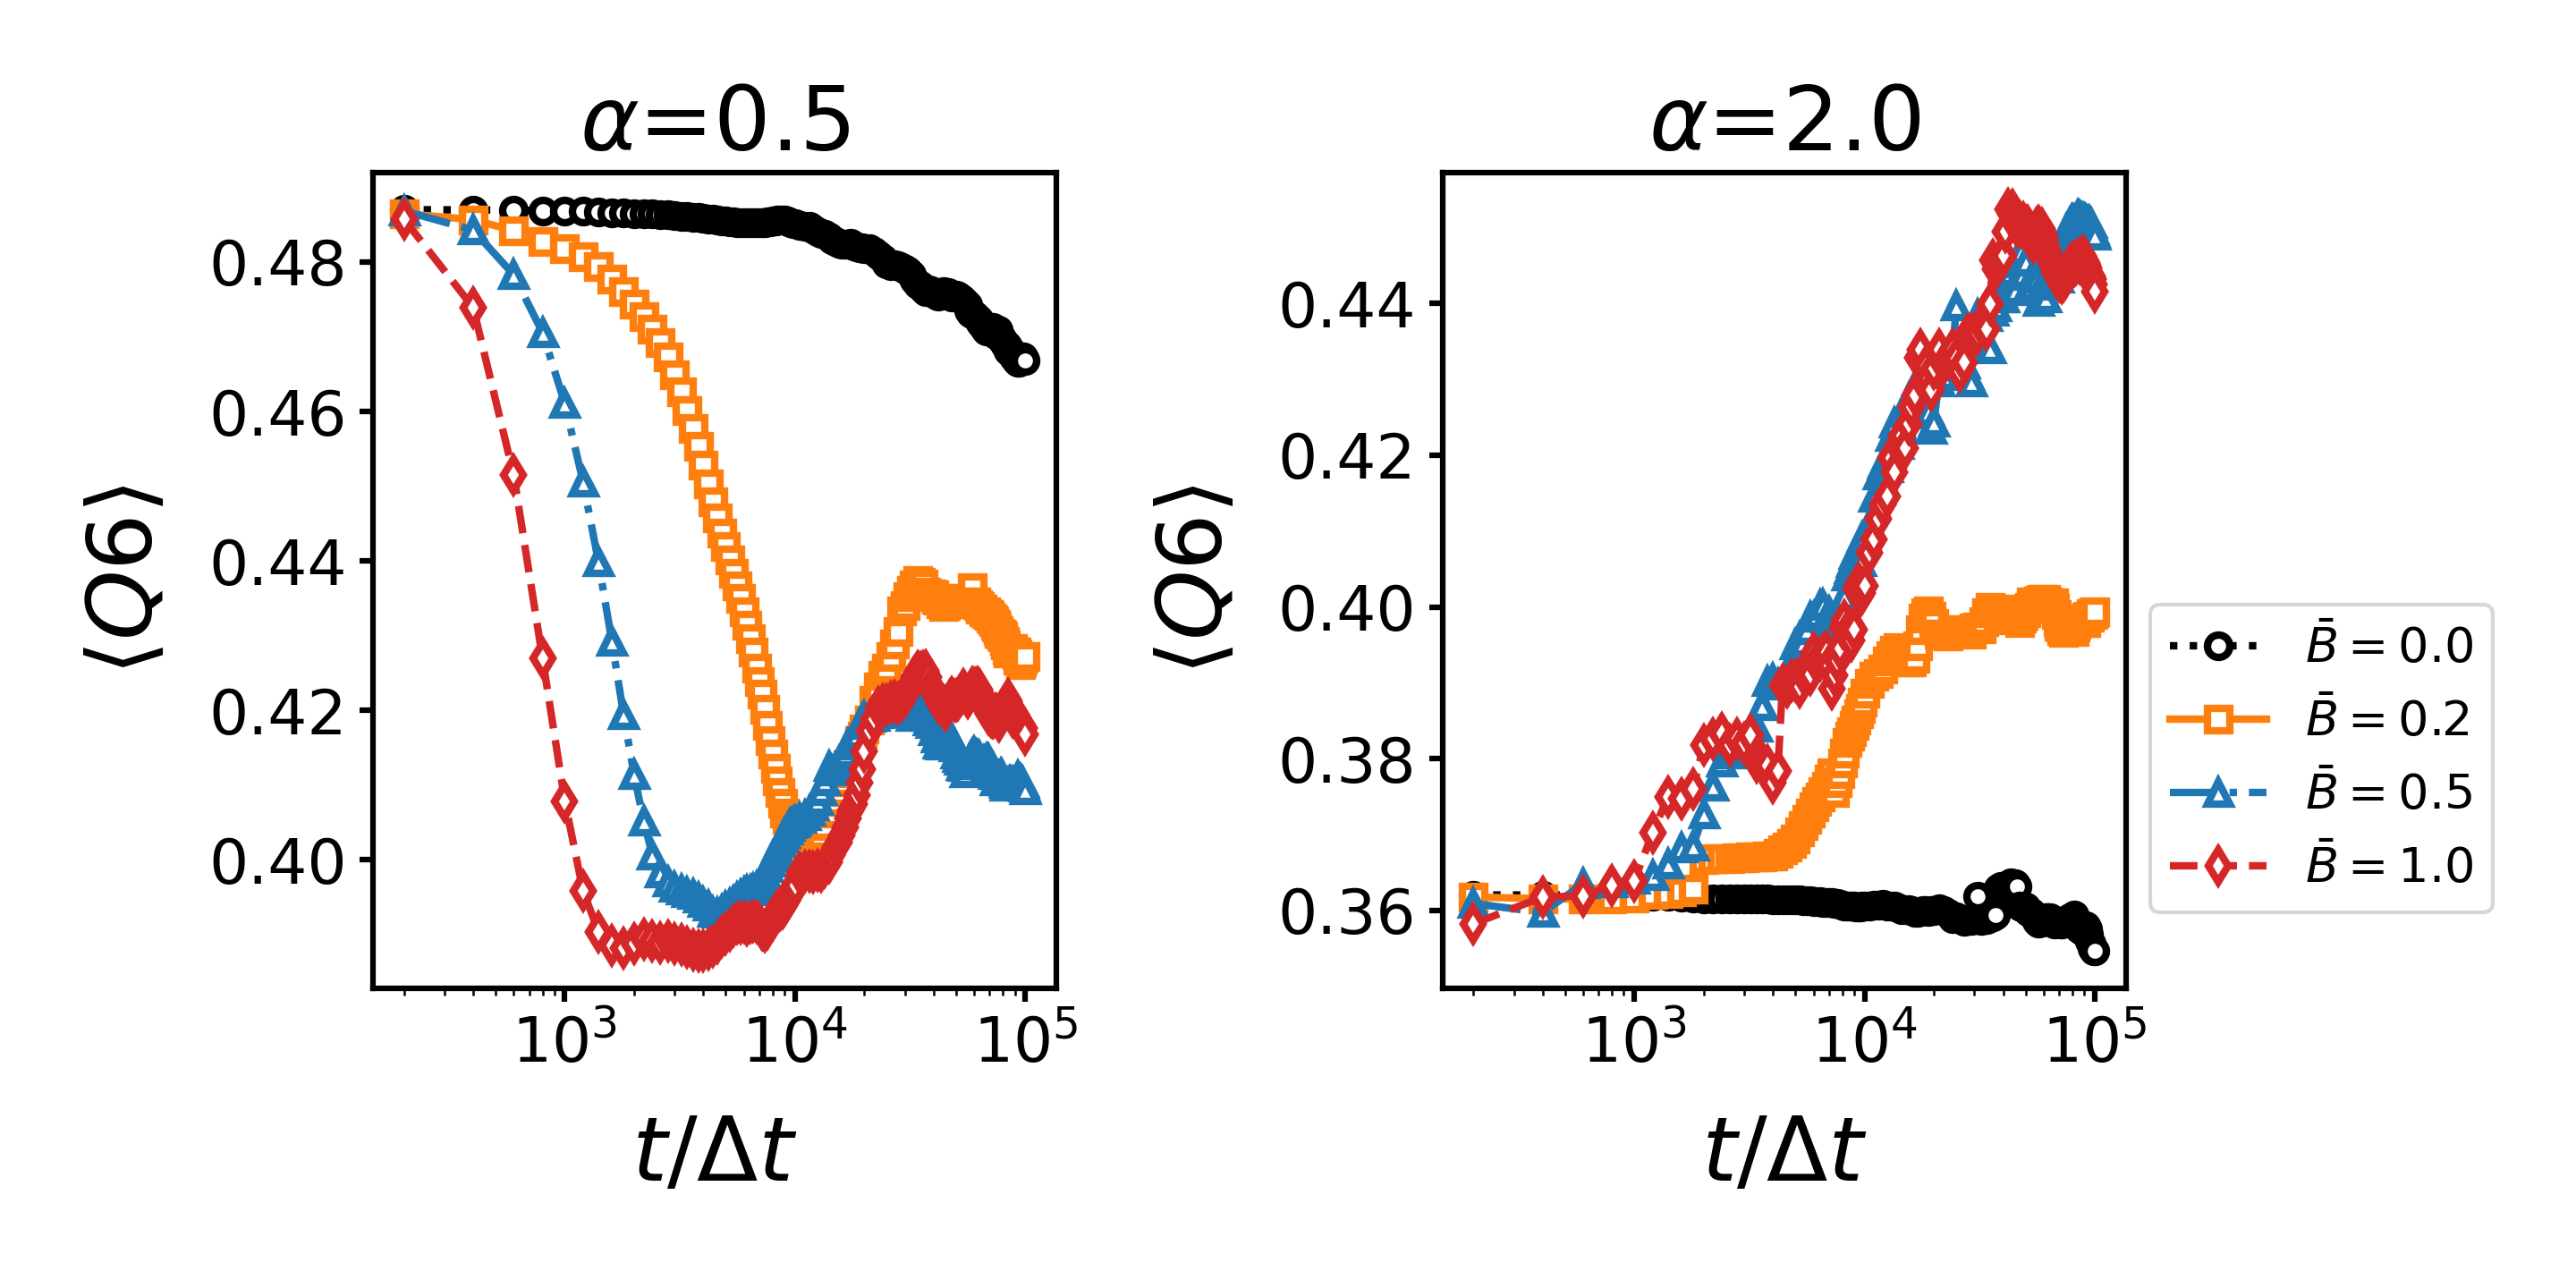
\includegraphics[scale=0.6]{../figures/results/paper2/Q6-field_on.png} 
    \caption{Plots of the time evolution of the six-fold Steinhardt bond order parameter \(\langle Q_6 \rangle\) for bijels 
             stabilized by oblate (left) and prolate (right) ellipsoidal particles under varying magnetic field strengths. The dynamics of interfacial ordering differ 
             significantly between particle morphologies with \(\langle Q_6 \rangle\) decreasing over time for oblate particles and increasing for prolate particles.} 
    \label{fig:Q6-field_on} 
\end{figure}

From Figure \ref{fig:Q6-field_on} the time evolution of \(\langle Q_6 \rangle\) can be qualitatively divided into three regimes;
an initial transition period, a plateau, and a final reordering or jamming phase.
For oblate particles, application of the magnetic field initially causes a sharp decrease in \(\langle Q_6 \rangle\), reflecting a disruption of the 
pre-existing interfacial order as particles begin to tilt and rearrange. This is followed by a plateau, during which ordering is temporarily suppressed 
as particles continue reorienting. Finally, \(\langle Q_6 \rangle\) begins to increase gradually, indicating partial recovery of local order as the system 
evolves toward a new jammed state. The rate of change of \(\langle Q_6 \rangle\) significantly decreases toward the end of the simulation, suggesting the onset 
of kinetic arrest. In contrast, for bijels stabilized by prolate particles, \(\langle Q_6 \rangle\) increases monotonically with time after the field is applied. The degree 
of ordering and the rate of increase both scale positively with magnetic field strength. The early stage is characterized by a modest rise in \(\langle Q_6 \rangle\), 
followed by a more rapid growth and eventual plateau, indicating progressive in-plane reordering of the particle monolayer as alignment along the field direction 
becomes dominant. The timing and extent of these regimes are also field-dependent with stronger fields result in earlier onset of ordering and higher final values 
of \(\langle Q_6 \rangle\).

The final value of \(\langle Q_6 \rangle\) is dependent on the applied magnetic field strength with oblate and prolate particles being affected by the field in
different ways. The trends match that characterized in Chapter 5, with oblate particles having lower hexagonal ordering upon application of a magnetic field
and prolate particles having a greater magnetic field. This was found to be due to oblate particles preferring to stack when magnetic fields are applied while
prolate particles order end to end ot side to side \cite{dabat_mesoscale_2018, eatson_capillary_2023}. This reordering can also explain why oblate particles
tilt out of the interface more than prolate particles.

Thus far, three key particle-scale phenomena have been characterized in response to the application of a magnetic field. The first is
particle alignment to the field direction, where both oblate and prolate ellipsoids reorient their major axes along the magnetic field vector. The second effect is
changes in particle tilt relative to the fluid interface, reflected in variations of the interface angle \(\langle \psi \rangle\), indicating out of interface 
reorientation driven by magnetic torque. Third, reorganization of the local particle monolayer, as captured by the evolution of the Steinhardt bond order parameter 
\(\langle Q_6 \rangle\), which reflects field-dependent disruptions and recoveries in particle ordering at the interface. Together, these processes 
drive the unjamming of the particle monolayer, causing coarsening of the fluid domains before the interface rejams in place with anisotropy dictated by the orientation
of particles to the magnetic field.

\subsection{Switching off an applied field}
\label{decreasing-the-applied-field}

Bijels are kinetically arrested systems whose long-term structural properties are governed by the stability and arrangement 
of the interfacial particle monolayer. Prior studies on responsive emulsions have shown that even after the removal of external 
stimuli, the microstructure often remains unchanged for extended periods due to the interfacial 
jamming of particles \cite{cui_stabilizing_2013}. Similarly, when assessing the kinetic arrest of bijels shown 
in Figure~\ref{fig:hysteresis_curve}, we observed that reducing or removing the magnetic field did not 
lead to a reversal of domain coarsening or particle realignment, suggesting an inherent structural resilience once the bijel 
has stabilized.

Gunther et al. also showed that bijels stabilized by ellipsoidal particles exhibited timescales 
of response distinct from bijels stabilized by spherical particle due to steric effects between ellipsoidal particles.
Therefore, this section will seek to understand to what extent the initial particle order affects the 
bijel's capacity to relax or restructure upon removal of the field. To explore this, 
we now examine the post-stimulus structural response of bijels formed under different field conditions 
\(\bar{B}_{\text{template}} = 0.0, 0.2, 0.5, 1.0\). After allowing each structure to fully stabilize under a 
constant magnetic field, we switch off the field and observe the subsequent time evolution of both the 
microstructure and interfacial particle behavior over a duration of \(t = 10^5 \Delta t\). This analysis aims to 
clarify the mechanisms that underpin the apparent irreversibility captured in the hysteresis response and further 
assess the role of the particles in bijel stability.

\begin{figure} 
\centering 
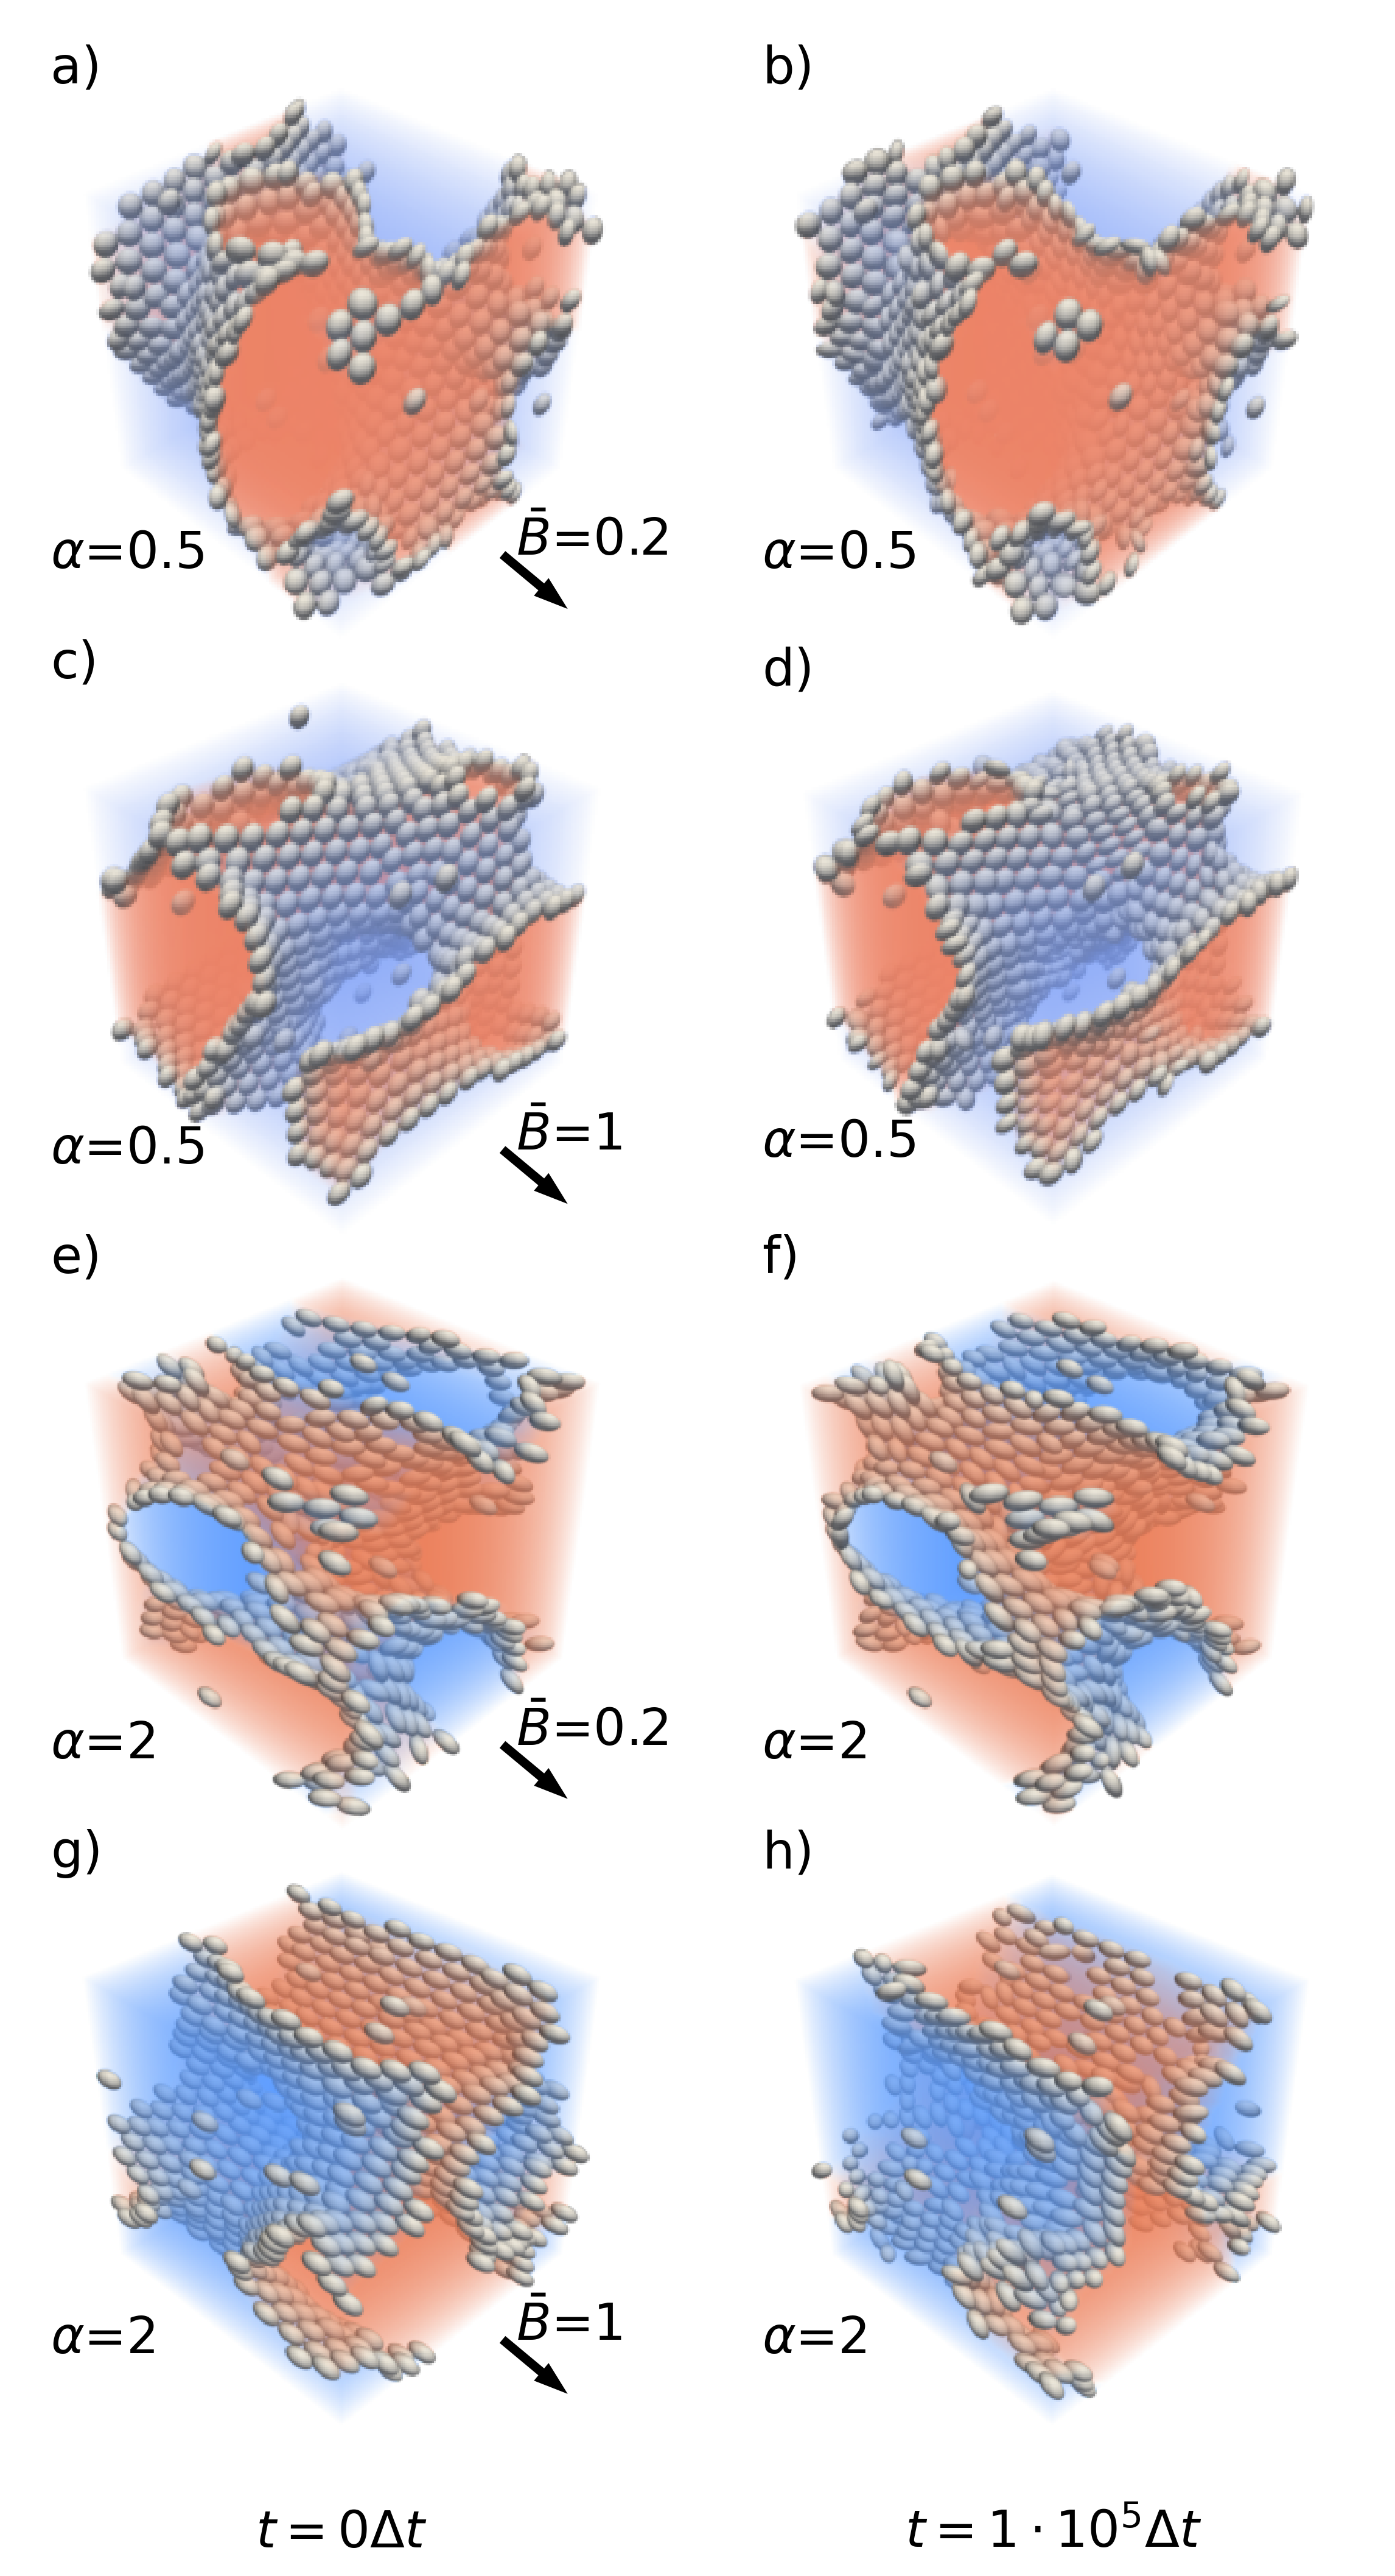
\includegraphics[scale=0.45]{../figures/results/paper2/microstructure_viz-field_down.png} 
\caption{Snapshots of bijels stabilized by prolate ellipsoids at 
         the initial and final time steps after the removal of an applied magnetic field. The top row corresponds to the case where 
         the field is reduced from \(\bar{B} = 0.2 \rightarrow 0.0\), and the bottom row from \(\bar{B} = 1.0 \rightarrow 0.0\)}
\label{fig:microstructure_viz-field_down}
\end{figure}

Figure \ref{fig:microstructure_viz-field_down} shows that in 
both cases, the bulk microstructure remains effectively unchanged over the course of the simulation, highlighting the 
kinetic stability and arrested nature of the bijel.
However, closer inspection of the interfacial particle arrangement reveals that in the
\(\bar{B}: 0.2 \rightarrow 0.0\) case, the particles retain a degree of orientational order, although slight deviations 
from the field-aligned configuration begin to emerge. In contrast, for \(\bar{B}: 1.0 \rightarrow 0.0\), where the 
initial nematic order was stronger, the particles exhibits more apparent disorganization by the final time step. This 
suggests that while the jammed interface resists large-scale rearrangement, there is a gradual relaxation of particle 
orientations in the absence of the aligning field. The extent of this relaxation correlates with the initial field strength when 
the field is removed. We probe the effect of these reorientations by calculating the time evolution of the domain size
in Figure \ref{fig:domain_size-field_down}

\begin{figure} 
\centering 
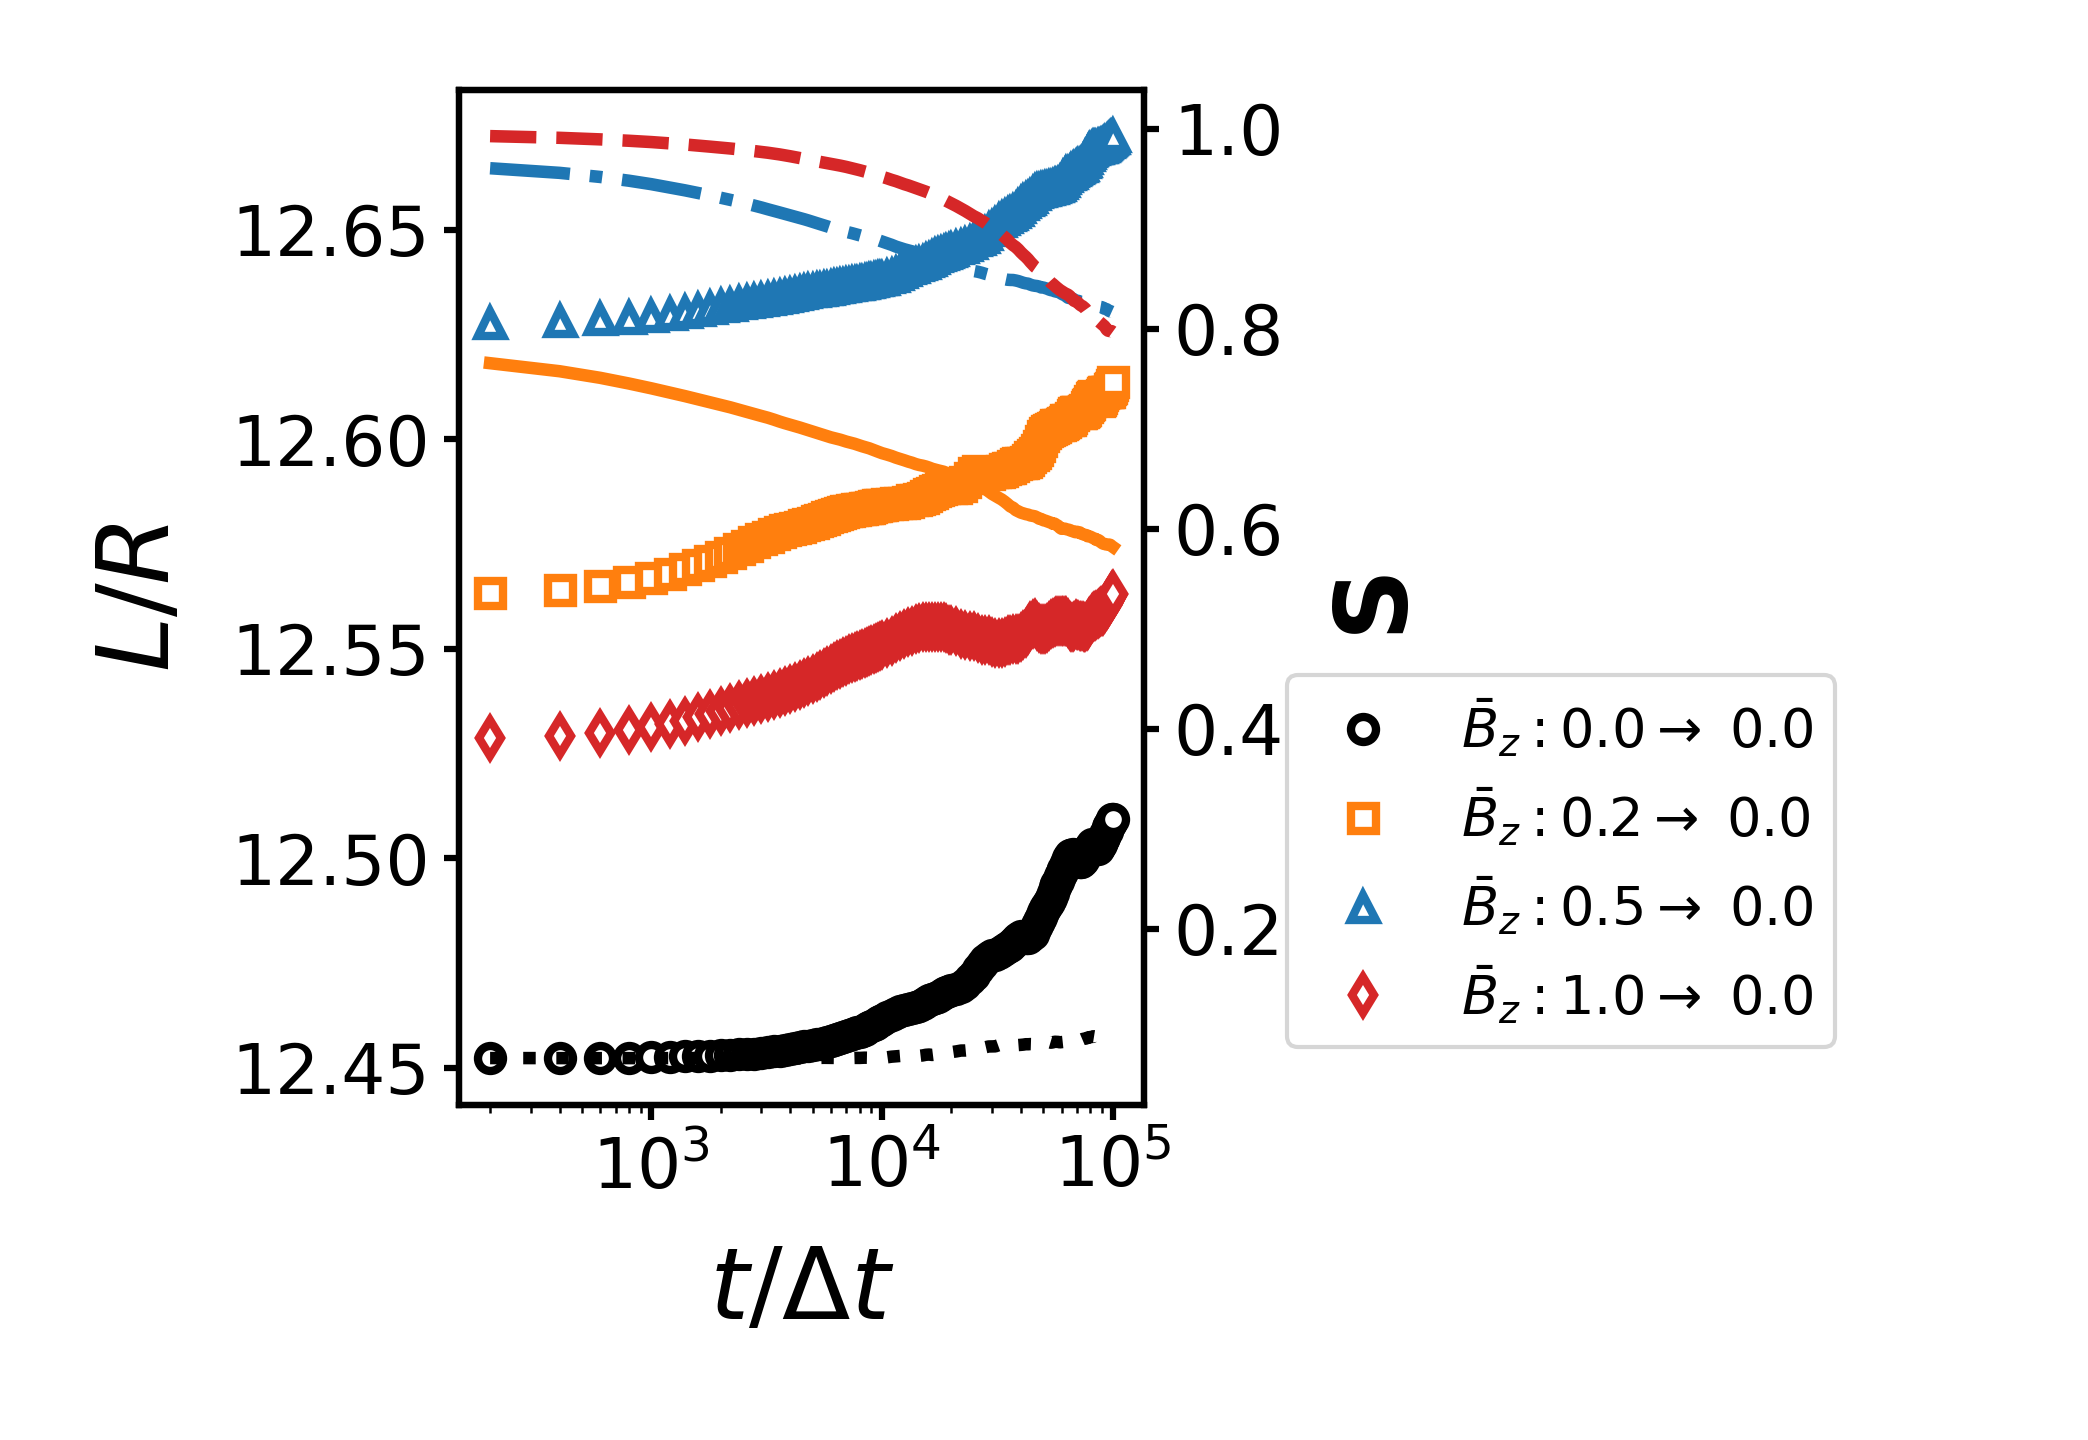
\includegraphics[scale=0.6]{../figures/results/paper2/domain_size-field_down.png} 
\caption{Plot of the spherically averaged domain size normalized with $R_p$ of the particle plotted over time. 
         Each color represents bijel templates made with different field strengths $\bar{B}$. We show that there is domain coarsening when the field 
         is switched off.} 
\label{fig:domain_size-field_down} 
\end{figure}

Figure~\ref{fig:domain_size-field_down} presents the time evolution of the normalized domain size (\(L/R\)) for bijels stabilized by oblate 
(left) and prolate (right) particles following the removal of an applied magnetic field. For all systems except oblate particle stabilized 
bijel with \(\bar{B}: 0.0 \rightarrow 0.0\), a modest degree of domain coarsening is observed. This slow, steady increase in domain size 
indicates that while the global microstructure remains largely intact, minor structural rearrangements may still occur post-stimulus, particularly 
at long timescales. This behavior is more prominent in prolate particle systems, suggesting that elongated particles 
may provide greater local flexibility for slight monolayer relaxation without disrupting the overall network.
A notable exception arises in the oblate \(\bar{B}: 0.0 \rightarrow 0.0\) case, which exhibits a pronounced 
increase in domain size at later times. These results reinforce the interpretation that bijel microstructure 
is resilient to field removal, with no meaningful reversal in the fluid once jamming has occurred even though local particle reorientation occurs.

\section{Conclusion}
% \section[Conclusion]{Conclusion\protect\footnote{Sections of this chapter appear in a manuscript submitted to Springerlink as part of the International Conference on Computational 
% Science (ICCS) 2025 in the Computing and Data Science for Materials Discovery and Design track, submission number 259 and is
% reproduced with permission of Palgrave Springer Nature.}}

In this work, we investigated how magnetic fields influence the structure and dynamics of bijels stabilized by magnetically responsive ellipsoidal particles. Motivated 
by the relevance of bijels in applications such as catalysis, membrane filtration, and drug delivery, we explored how external stimuli can enable in-situ control over 
microstructure in these systems. Using hybrid Lattice Boltzmann-Molecular Dynamics simulations, we characterized the structural response of formed bijels by investigating
the effect of applying a magnetic field and the initial microstructure on the structural response characterized. We first demonstrated that bijels subjected to increasing 
magnetic field strength exhibit kinetic arrest in its structural response, where the domain size increases with field application but does not revert upon field removal.

When investigating the effect of the application of magnetic fields, our results revealed that applying magnetic fields post-formation induces domain coarsening up to 5\%, with 
field-induced anisotropy dependent on particle shape. These changes arise from particle reorientation to the field, followed by 
local unjamming and interfacial rearrangement before re-jamming occurs, as characterized using the average interface angle of the particles and the 
Steinhardt bond orientational order parameter. In contrast, removing the magnetic field had little effect 
on bijel structure. Domain size and anisotropy remained largely unchanged, regardless of initial particle order. While minor relaxation in particle alignment was observed, 
capillary forces alone were insufficient to drive significant structural reorganization.

These results show that rapid coordinated reorientation of the particle stabilizers is necessary to induce structural response in bijels. This is illustrated through structural response
of bijels occurring upon application of the field, causing rapid realignment of particles to the applied field direction while slow realignment of particles away from
the field when switching the field off generated no meaningful changes in the microstructure.

While our simulations offer insights into the tunability of bijels, they were limited to a single set of fluid and particle parameters. Future work could explore the 
effects of particle size, volume fraction, interparticle forces, and field orientation or gradients, all of which may unlock additional control over bijel structure.
Ultimately, this study establishes a foundation for stimuli-responsive bijels, showing how particle-level interactions and monolayer dynamics translate into controllable, 
application-relevant changes in material microstructure.